% ============================================================
% Multimodal Breast Cancer Molecular Subtyping Paper
% Target: IEEE Journal of Biomedical and Health Informatics (JBHI)
% Format: Two-column, single-spaced, max 12 pages
% ============================================================
\documentclass[10pt,journal,compsoc,twocolumn]{IEEEtran}

% ---- Essential Packages ----
\usepackage{amsmath,amssymb}
\usepackage{graphicx}
\usepackage{booktabs}
\usepackage{multirow}
\usepackage{array}
\usepackage{caption}
\usepackage{subcaption}
\usepackage{xcolor}
\usepackage{hyperref}
\usepackage{etoolbox}
\usepackage{url}
\usepackage[numbers,sort&compress]{natbib}

% ---- Table fitting: uniform \small size; scale down only if a table
%      still exceeds the IEEE single-column width ----
\AtBeginEnvironment{table}{\small}
\newcommand{\fitcol}[1]{%
  \resizebox{\ifdim\width>\columnwidth\columnwidth\else\width\fi}{!}{#1}}

% ---- Custom Colors ----
\definecolor{accentblue}{RGB}{31,119,180}
\definecolor{accentorange}{RGB}{255,127,14}
\definecolor{accentgreen}{RGB}{44,160,44}

% ---- Header/Title Info ----
\title{Label-Space Mismatch Distorts Cross-Cohort Evaluation in Breast Cancer Molecular Subtyping}

\author{
\IEEEauthorblockN{Suxing Liu}
\IEEEauthorblockA{School of Digital Arts, Jiangxi Arts \& Ceramics Technology Institute,\\
Jingdezhen 33001, China\\
Email: liushuxing8888@student.usm.my\\
ORCID: 0009-0005-9893-4163\\
(Corresponding author)}
\and
\IEEEauthorblockN{Zhijian Zheng}
\IEEEauthorblockA{University of Alabama,\\
Tuscaloosa, AL, USA}
\and
\IEEEauthorblockN{Jiahao Wang}
\IEEEauthorblockA{School of Computing, Universiti Sains Malaysia,\\
11800 USM Penang, Malaysia}
}

\begin{document}

\maketitle

\begin{abstract}
Cross-cohort evaluations can be misleading when datasets use different annotation standards, as demonstrated here in breast cancer molecular-subtype classification, where METABRIC labels include six classes and PAM50 annotations include five intrinsic subtypes. The METABRIC multimodal analysis included 1,369 patients with aligned data, split into training (n=958), validation (n=205), and test (n=206) sets. External label-space analyses used mRNA classifiers on TCGA-BRCA (n=987) and GSE21653 (n=266). We compared uncorrected predictions with restriction to the five PAM50 classes and expectation-maximisation (EM) prior correction, without using target labels. Uncorrected accuracy was 73.76\% on TCGA-BRCA, similar to 73.8\% on the METABRIC test set. Six-class macro F1 was 0.585 on TCGA-BRCA, compared with 0.702 when scored over its five annotated classes. On GSE21653, uncorrected accuracy was 63.16\%. Restricting predictions to PAM50 classes and applying EM correction increased accuracy to 80.65\% on TCGA-BRCA and 74.06\% on GSE21653. These are changes in evaluation rules, not improvements in the model's learned representation. Without annotation-space information, unconstrained EM assigned the absent claudin-low class a prior of 0.0751 on TCGA-BRCA, and no tested detector identified absent classes reliably across covariate and prior shift: re-scored under the standard empty-set convention, the original uncalibrated rule has the highest F1 and exact-set match of the six tested (0.786 and 0.550), but its mean F1 on cohorts with a truly absent class falls to 0.543 at the highest covariate shift, while its calibrated replacements flag clean cohorts in 73 and 87 of 120 cases. The internal multimodal advantage did not survive external validation: in a reduced three-layer space shared by both cohorts (412 mRNA genes, 209 measured methylation genes, 10 clinical fields; n=694), adding methylation lowered TCGA accuracy by 1.9 points, the harmonized clinical block gained 2.4 points on the METABRIC test set but moved external accuracy by at most 0.3 points, and no configuration differed significantly from mRNA alone (paired McNemar, $p = 0.13$ to $1.00$). The best internal model rested on 59 METABRIC-specific clinical dimensions that have no external counterpart. Survival discrimination was similar across the external cohorts (C-index 0.577 and 0.584). In GSE20194 (n=278), the genomic panel did not significantly improve pCR prediction over clinical variables ($\Delta$AUC = +0.0045; 95\% CI, -0.060 to +0.061). In the studied cohorts, cohort-level performance is not directly comparable when annotation standards define different label spaces. The target cohort's allowed labels should be established before computing comparative metrics; in these experiments, unlabeled predictions alone did not identify the absent class.
\end{abstract}

\begin{IEEEkeywords}
Breast cancer, molecular subtyping, PAM50, label-space mismatch, label shift, cross-cohort evaluation, multimodal integration
\end{IEEEkeywords}

\section{Introduction}
Breast cancer is a heterogeneous disease characterized by distinct molecular subtypes that differ in gene expression patterns, clinical behavior, and treatment response \cite{perou2000molecular}. The PAM50 classification system defines five intrinsic subtypes: Luminal A, Luminal B, HER2-enriched, Basal-like, and Normal-like \cite{parker2009supervised}. Claudin-low is a separate designation based on additional markers \cite{prat2010phenotypic}. Accurate subtyping can inform treatment selection and prognosis assessment \cite{prat2014research}.

Current approaches to breast cancer subtyping predominantly rely on single data modalities. The Prosigna (PAM50) test uses only gene expression data \cite{parker2009supervised}, while clinical risk calculators such as Nottingham Prognostic Index use only clinicopathological features \cite{haybittle1982prognostic}. However, breast cancer biology is driven by the interplay of genomic, epigenomic, and clinical factors. DNA methylation patterns, for instance, play a crucial role in regulating gene expression in breast cancer \cite{pasculli2018epigenetics}, and clinical variables such as ER/PR/HER2 status carry independent prognostic information \cite{goldhirsch2013personalizing}.

Multimodal learning has emerged as a promising paradigm for cancer classification, with studies demonstrating that integrating multiple data types can improve prediction accuracy and biological understanding \cite{wang2014similarity, chaudhary2018deep, sharifinoghabi2019moli}. However, several challenges remain: (1) many multimodal approaches require large training datasets that are unavailable for rare cancer subtypes; (2) models trained on one profiling platform often fail to generalize to data from different platforms; and (3) the relative contributions of different modalities are poorly understood.

Label-shift methods provide established tools for estimating or correcting changes in class prevalence from unlabeled target predictions. These include black-box shift estimation, EM-based prior adjustment, regularized adaptation, calibration-aware estimation, and methods for open-set or generalized label shift \cite{lipton2018detecting,azizzadenesheli2019regularized,saerens2002adjusting,alexandari2020maximum,garg2020unified,garg2022open,tachetdescombes2020domain}. These methods address changes in class proportions within a specified label space. They do not by themselves establish that source and target annotation standards define the same set of classes. We examine that distinction in breast cancer molecular-subtype evaluation rather than proposing a new label-shift algorithm.

We use a multimodal METABRIC model as an internal reference and focus the cross-cohort analysis on its mRNA classifier, the feature block available across cohorts. The central question is whether apparent performance differences can be interpreted before reconciling the target cohort's annotation space. We quantify the effect of restricting predictions to the five PAM50 classes, separate that operation from prior correction, and test whether absent classes can be inferred from unlabeled predictions. Survival discrimination and multimodal feature attribution provide secondary analyses.

The analysis raised a question about a lower accuracy observed in one external cohort. The target cohort used PAM50 annotations, whereas the METABRIC model had six output classes, including claudin-low. Predictions assigned to a class excluded by the target annotation standard cannot be correct under that evaluation. Section~\ref{sec:labelspace} measures the effect of reconciling the label space and compares it with prior correction. It also evaluates whether the absent class can be identified from unlabeled target predictions.

Our key contributions are:
\begin{enumerate}
  \item We quantify how a mismatch between the six-class training label space and the five-class PAM50 annotation space changes cross-cohort metrics, separately from prior correction (Section~\ref{sec:labelspace});
  \item Using the annotation-standard fact that claudin-low is not a PAM50 subtype, without target labels, we change accuracy from 73.76\% to 80.65\% on TCGA-BRCA and from 63.16\% to 74.06\% on GSE21653. These are evaluation-rule changes, not retraining gains;
  \item We show that the tested unlabeled-data procedures do not reliably identify the absent class. Unconstrained EM retains an estimated claudin-low prior of 0.0751 on TCGA-BRCA, and two tested detectors do not reliably recover the annotation space;
  \item We report a negative result for cross-modal attention fusion. Capacity sweeps, regularization, and self-supervised pretraining did not bring the tested architecture to the linear reference, and its internal gains did not transfer;
  \item A systematic evaluation of modality combinations, demonstrating that clinical + mRNA + methylation outperforms all five modalities, together with SHAP-based modality attribution and survival analysis confirming significant prognostic stratification.
\end{enumerate}

\section{Related Work}
\label{sec:related}

\subsection{Multimodal and Multi-Omics Learning in Cancer}
Fusing heterogeneous molecular and clinical data is now a standard approach in computational oncology, and deep architectures have been applied to diagnosis, prognosis and treatment selection across tumour types \cite{tran2021deep,poirion2021deepprog,moon2023machine,jiang2024autosurv}. The dominant design in recent work is graph-based: multi-omics profiles are represented as graphs and combined through attention or message passing \cite{lin2026moagnn,fan2026cmgl,tan2025amogel,dou2025mogcan,zhang2025hallmarkgraph,tanvir2024mogat,xiao2023graph,zhang2025multiomics,li2024graphnn}, often with hierarchical or multi-view objectives \cite{ren2024classifying,yang2024multimodal}. Alternative fusion strategies include tensor and stacked fusion \cite{zhang2024msfn}, contrastive fusion \cite{liu2023attentionbased}, and autoencoder-based joint embedding \cite{benkirane2023customics,chai2021integrating}. For breast cancer specifically, attention-based fusion has been applied to predicting neoadjuvant chemotherapy response \cite{zhang2025attentionbased}, and multimodal systems have been built for pathological complete response and survival prediction \cite{mao2025a,cheng2026aligned,jia2026dynamic}.

These methods are typically assessed by internal cross-validation, and reported gains over single-modality baselines are often a few points. Recent reviews note that fusion architectures are rarely validated on cohorts drawn from a different source than the training data, and that the field lacks shared evaluation protocols \cite{steyaert2023multimodal,li2024a,huang2024classifying,kibria2026decoding}. Our study is complementary to this line: we do not propose a new fusion architecture, and the one we tested did not beat a linear reference (Section~\ref{sec:route_a}). Instead we examine what happens to the \emph{evaluation} of such models when the target cohort's annotation standard differs from the source's.

\subsection{Label Shift, Domain Adaptation and Calibration}
Distribution shift between training and deployment cohorts has a substantial literature, of which the closest strand to our problem is label shift: the class proportions change while the class-conditional distributions do not. Early work estimated target priors from unlabelled predictions by expectation-maximisation \cite{saerens2002adjusting}, and the procedure we use is a direct descendant of that estimator. Subsequent work has refined estimation and correction \cite{garg2022open,roberts2022unsupervised,liu2021scuda,stan2024unsupervised,mahapatra2024alfredo}, extended it to open-set and generalised settings where the label spaces themselves may differ \cite{popordanoska2024lascal,yang2025a1,yoshida2025classprior,volpi2025leap,gilet2023softmin,nakajima2022positiveunlabeled}, and connected it to test-time and source-free adaptation \cite{yang2022dltta,chen2025vpsfda,wang2022embracing,bandyopadhyay2021cryoshift,park2021transfer,lai2023domainaware}. Calibration is the natural companion question: whether a corrected model's probabilities remain faithful to observed frequencies, which we address with Brier and ECE in Supplementary Section~S3.

This literature treats the label space as given and estimates only the priors within it. Open-set label shift is the nearest exception \cite{popordanoska2024lascal,yang2025a1}, but it still assumes the target's label space is discoverable from data. Our negative result speaks to that assumption: when a class is genuinely unrepresentable under the target's annotation standard, the tested prior-estimation and detection procedures did not recover the fact, and the correction therefore has to be supplied from cohort documentation rather than inferred.

\subsection{PAM50 Annotation and Cross-Platform Concordance}
The PAM50 intrinsic subtypes are defined by a 50-gene expression signature \cite{parker2009supervised}, but their assignment is not perfectly reproducible. Studies report discordance between PAM50 calls and immunohistochemistry-based surrogate definitions \cite{phakathi2023pam50,lopeztarruella2023correlation,sayed2026immunohistochemistry}, between primary and metastatic lesions \cite{jrgensen2021pam}, and across populations \cite{desalegn2022intrinsic,hohmann2025molecular}. Reproducibility of the assay itself has been quantified and found to be limited by intratumoral heterogeneity \cite{hurson2023reproducibility,dixpeek2023discordance}. Methodological work has sought to stabilise calls through rank-based normalisation \cite{kandan2025rank}, improved implementations \cite{rajkumar2025enhanced}, and derived scores designed to transfer across platforms \cite{denegreirosbotan2026corepam}. Batch and preprocessing effects on subtyping are themselves an active concern \cite{wu2023on6,chen2022pathomic,rojasvelazquez2024methodology,van2024a,ng2023the,mann2021artificial,zhang2021machine}.

This body of work establishes that annotation disagreement of the kind we study is real and consequential, but it addresses disagreement \emph{within} a shared label space -- two assays disagreeing about which of the five PAM50 subtypes a tumour is. The failure we examine is one level up: the two cohorts do not share a label space at all, because one annotates a sixth class the other's standard cannot express. Our supplementary sweep shows that this class of mismatch is governed by the prior mass of the absent class, and that its most common real form -- a class folded into a neighbouring label rather than dropped -- is also its most damaging.

\section{Methods}

\subsection{Data Collection and Preprocessing}

\subsection{METABRIC Dataset}
The Molecular Taxonomy of Breast Cancer International Consortium (METABRIC) dataset \cite{curtis2012genomic} was used as the primary development cohort. The source cohort contained 1,974 patients with PAM50 annotations. The analysis set comprised 1,369 patients retained after aligning patient identifiers across the clinical, mRNA, copy-number, methylation, and mutation records used in preprocessing. The 1,369-patient analysis set was split into training, validation, and test subsets. Five-fold cross-validation estimates were computed within the training subset (n=958), not across the full aligned analysis set.

Clinical features were encoded from 22 categorical and continuous variables including age at diagnosis, tumor size, tumor stage, ER/PR/HER2 status, and treatment history. Categorical variables were one-hot encoded, and continuous variables were Z-score standardized, yielding 69 clinical feature dimensions. mRNA expression data were filtered to 412 genes (subset of the 488 available genes matching the TCGA gene panel), and DNA methylation comprised 232 CpG probes selected by variance ranking.

The analysis set was split into training (n=958, 70\%), validation (n=205, 15\%), and test (n=206, 15\%) sets using stratified random sampling to preserve subtype proportions. Class distribution in the training set: Luminal A (35.7\%), Luminal B (23.9\%), HER2-enriched (12.5\%), claudin-low (9.5\%), Basal-like (10.4\%), and Normal-like (7.9\%).

\subsection{TCGA-BRCA External Validation Dataset}
The Cancer Genome Atlas Breast Cancer (TCGA-BRCA) cohort \cite{cancer2012comprehensive} was used for external validation. From the Firehose Legacy study (1,108 patients), we obtained RNA-seq V2 expression data (1,100 samples) and PAM50 annotations (987 samples with 5 subtypes; claudin-low not annotated). Survival data were available for 966 patients with 133 death events (13.8\% event rate).

Gene expression was mapped from the 412-gene METABRIC panel using Entrez Gene IDs via the cBioPortal API. Within each platform, expression values were rank-transformed and normalized using the inverse normal CDF to achieve cross-platform comparability:
\begin{equation}
  x_{ij}^{\text{norm}} = \Phi^{-1}\left(\frac{\text{rank}(x_{ij})}{n_j + 1}\right)
  \label{eq:rank_norm}
\end{equation}
where $\Phi^{-1}$ is the inverse normal CDF and $n_j$ is the number of samples in platform $j$. This within-platform normalization preserves relative sample ordering while removing platform-specific distributional differences.

\subsection{GEO External Cohorts}
GSE21653 was obtained from the Gene Expression Omnibus (GEO). It comprises 266 tumors profiled on GPL570 (Affymetrix Human Genome U133 Plus 2.0), with PAM50 subtype calls and disease-free survival records. Of the 412 genes in the METABRIC panel, 369 mapped to this platform. When multiple probes mapped to one gene, the probe with the highest mean expression was retained. Expression values were normalized within the cohort using the rank-based procedure above.

GSE20194 was obtained from GEO for the secondary pathological complete response (pCR) analysis. The cohort included 278 patients treated with neoadjuvant chemotherapy, of whom 56 achieved pCR and 222 had residual disease. The series was profiled on the Affymetrix Human Genome U133A platform (GPL96); 276 genes from the 412-gene panel mapped to this platform. The published pCR labels were used only as the outcome for this secondary analysis.

\subsection{Multimodal Feature Engineering}
We engineered features from five modalities:
\begin{enumerate}
  \item \textbf{Clinical} (69d): One-hot encoded categorical variables (e.g., ER status, HER2 status, tumor stage, surgery type, treatment history) with Z-score standardized continuous variables (age, tumor size, lymph node count, NPI).
  \item \textbf{mRNA expression} (412d): Microarray expression values for 412 genes, Z-score standardized.
  \item \textbf{Copy number alteration} (256d): Top 256 genes by variance from SNP 6.0 array, Z-score standardized.
  \item \textbf{DNA methylation} (232d): Beta values for 232 CpG probes selected by variance, Z-score standardized.
  \item \textbf{Somatic mutations} (173d): Binary indicators for 173 genes with at least one mutation in the cohort.
\end{enumerate}

Total feature dimensions across all modalities: $69 + 412 + 256 + 232 + 173 = 1{,}142$.

\subsection{Model Development}

\subsection{Logistic Regression}
Multinomial logistic regression was chosen as the primary classifier due to its strong performance on small-sample, high-dimensional data and inherent interpretability. The model uses the softmax function:
\begin{equation}
  P(y = k \mid \mathbf{x}) = \frac{\exp(\mathbf{w}_k^\top \mathbf{x} + b_k)}{\sum_{j=1}^{K} \exp(\mathbf{w}_j^\top \mathbf{x} + b_j)}
  \label{eq:softmax}
\end{equation}
with $L_2$ regularization controlled by parameter $C$. We evaluated $C \in \{0.001, 0.01, 0.1, 1.0, 10.0\}$, with $C = 0.01$ selected by cross-validation. Estimators were implemented with scikit-learn \cite{pedregosa2011scikit}.

\subsection{Comparison Models}
We compared logistic-regression regularization variants and a sigmoid-calibrated model with Random Forest (300 trees), XGBoost, LightGBM, CatBoost, Extra Trees, soft-vote ensembles, and Transformer variants \cite{vaswani2017attention}. The Transformer model used five modality-specific linear projections feeding into a two-layer encoder ($d_{\text{model}}$=64, four attention heads) with a classification head (174K parameters).

\subsection{Ensemble and Cascade Methods}
We explored: (1) soft-vote ensemble of LogReg + GBDT + XGBoost; (2) a two-stage cascade where LogReg classifies high-confidence samples and a Transformer handles low-confidence samples; and (3) a Guided Transformer where LogReg probability outputs serve as a soft prompt token for cross-modal attention.

\subsection{Evaluation Protocol}

\subsection{Classification Metrics}
Primary metrics: accuracy and macro-averaged F1-score. Secondary metrics: per-class precision, recall, and F1-score. Statistical significance of model differences was assessed using McNemar's test on the held-out test set.

\subsection{Survival Analysis}
Predicted subtype probabilities were used as covariates in a Cox proportional hazards model:
\begin{equation}
  h(t) = h_0(t) \exp\left(\sum_{k=1}^{K-1} \beta_k \hat{p}_k\right)
  \label{eq:cox}
\end{equation}
where $\hat{p}_k$ is the predicted probability for subtype $k$ (Luminal A as reference), and $h_0(t)$ is the baseline hazard. Discrimination was assessed using the concordance index (C-Index) at 3-year, 5-year, and 10-year time horizons. Kaplan-Meier survival curves were compared using the log-rank test.

\subsection{Interpretability Analysis}
SHAP (SHapley Additive exPlanations) \cite{lundberg2017unified} with the LinearExplainer was used to quantify feature importance. The explainer is exact rather than approximate here: the fitted classifier is multinomial logistic regression, a linear model, and for a linear model the LinearExplainer computes the Shapley values in closed form from the coefficients and the background distribution. This is not a convenience fallback for a nonlinear model but the estimator matched to the hypothesis class. Modality contribution was computed as the mean absolute SHAP value aggregated across all features within each modality. The analysis was performed on a 300-sample subset of the training data.

\subsection{Label-Space Reconciliation and Prior Correction}
\label{sec:methods_shift}

Because the training cohort carries six classes and the external cohorts carry five, the classifier's output space must be reconciled before any accuracy is computed. We define a \emph{label-space mask} $m \in \{0,1\}^K$ with $m_k = 0$ for any class $k$ that the target cohort's annotation standard cannot emit. For PAM50-annotated cohorts this mask is fixed by the annotation standard alone. Claudin-low is not one of the five PAM50 intrinsic subtypes \cite{parker2009supervised}, so the mask is \emph{independent of the target labels}. This distinction is load-bearing and we state it explicitly: deriving the mask from $\text{unique}(y_{\text{target}})$ would leak the labels and inflate the result, so every number reported in Section~\ref{sec:labelspace} uses the hard-coded annotation mask.

We compare four estimators within each target cohort. They share the same fitted classifier and feature set within that cohort. TCGA-BRCA uses all 412 mapped genes. GSE21653 uses the 369 genes mapped to GPL570, with the source classifier refitted on the corresponding METABRIC columns:

\begin{enumerate}
  \item \textbf{base}: $\arg\max_k p_k$, with no reconciliation (the conventional protocol);
  \item \textbf{mask\_only}: zero the masked columns and renormalise;
  \item \textbf{em\_pam50}: expectation-maximisation prior correction \cite{saerens2002adjusting} over the full $K$-class space, with masked columns fixed at zero throughout;
  \item \textbf{em\_full}: the same EM procedure with \emph{no} mask, meaning it receives no label-space knowledge whatsoever.
\end{enumerate}

The source prior is the METABRIC training composition. EM updates the target probabilities and class priors as follows:
\begin{align*}
p_k^{(t+1)}(x) &\propto p_k^{(t)}(x)\, \pi_k^{(t)} / \pi_k^{(0)}, \\
\pi^{(t+1)} &= \mathbb{E}_x[p^{(t+1)}(x)].
\end{align*}
Iterations stop when the prior changes by less than $10^{-6}$. The contrast between \textbf{em\_pam50} and \textbf{em\_full} isolates the value of the label-space fact. Both use identical unlabelled target predictions, but only one is given the structurally impossible classes.

Gains are reported with a paired bootstrap ($n_{\text{iter}} = 2000$, resampling target samples and recomputing both endpoints), and a split-half transductive check confirms the correction does not depend on how the target is partitioned.

\subsection{Controlled Simulation of Mismatch}
\label{sec:methods_sim}

To separate the contributions of label-space mismatch from ordinary prior shift we simulate targets under a full factorial design: label-space mismatch $n_{\text{absent}} \in \{0,1,2\}$, covariate shift $\in \{0.0, 0.4, 0.8\}$, and prior shift $\in \{\text{false}, \text{true}\}$, with 20 seeds per cell and $n_{\text{target}} = 1000$. A class is treated as absent when its target prevalence falls below $\tau_{\text{absent}} = 0.02$ or below $\tau_{\text{ratio}} = 0.10$ of its source prevalence. Each cell reports accuracy with no correction, with an oracle label-space mask, and with a mask estimated from the target.

That design removes only the rarest classes and only removes them completely, which is the pattern realised by claudin-low. Because a reader should not have to assume that the mildest instance is representative, we run a second, larger sweep over two further axes (Supplementary Section~S5). The first varies \emph{which} class is absent across all six and all fifteen pairs, so a mismatch involving a common or confusable subtype is covered. The second varies \emph{how} it is absent, distinguishing three patterns seen in practice: a class dropped outright, a class under-ascertained rather than absent (prevalence scaled to $\tau_{\text{ratio}}$ of source), and a class \emph{merged} into a neighbour's label -- claudin-low recorded as Basal-like, or Luminal B recorded as Luminal A, which is the most common form of annotation disagreement between cohorts.

\subsection{Geometric Absence Detection}
\label{sec:methods_detector}

We also asked whether the absent class could be identified from unlabelled predictions alone, without being told. We built a detector on the geometry of the target probability simplex: for candidate absent set $S$, measure the ratio of observed mass to source-expected mass on the columns in $S$, and flag $S$ when that ratio exceeds a threshold $\tau$. The threshold was calibrated on null data (no truly absent class) at level $\alpha = 0.05$, taking the 95th percentile of the maximum ratio statistic under the null. This calibration is what makes the detector a fair test rather than a tuned one: $\tau^*$ is chosen so that a cohort with no absent class is flagged at most 5\% of the time.

\subsection{Generative Model-Selection Detection}
\label{sec:methods_lrt}

Because a hand-calibrated threshold is the obvious objection to the detector above, we also tested a mechanism that sets no threshold at all. Here the target sample is modelled as $p(x) = \sum_{k \in M} \pi_k \, \mathcal{N}(x ; \mu_k, \Sigma)$, with the component means and the shared covariance estimated from the \emph{source} labels and the mixture weights $\pi$ fitted on the unlabelled \emph{target} by expectation-maximisation over an allowed label space $M$. Candidate label spaces are all subsets of size 4, 5, or 6. This includes every configuration with zero, one, or two absent classes. The winner is the subset minimising the Bayesian information criterion $\text{BIC} = -2\log L + (|M| - 1)\log n$, so the complexity penalty, rather than a tuning constant, is what controls the trade-off; predictions are formed on a 40-component PCA projection of the standardised features. No target labels are used at any point.

\section{Results}

\subsection{Modality Selection Reveals Optimal Feature Combination}
\label{sec:modality}

Systematic evaluation of modality combinations (Table~\ref{tab:modality_ablation}) revealed that adding more modalities did not always improve performance. The clinical + mRNA + methylation model (713 dimensions) achieved 79.0\% validation accuracy, 3.4 percentage points above the full five-modality model (75.6\%). In cross-validation, adding CNA alone or mutation alone to the selected three-modality model reduced accuracy by 2.3 and 2.0 points, respectively. The full five-modality model scored 72.4\%, 2.9 points below the selected model.

\begin{table}[htbp]
\centering
\caption{Modality-combination ablation on the METABRIC validation set (n=205). Five-fold cross-validation results use the training subset (n=958). The clinical + mRNA + methylation model exceeds the all-modality model by 3.4 percentage points on the validation split.}
\label{tab:modality_ablation}
\fitcol{%
\begin{tabular}{lccc}
\toprule
\textbf{Modality Combination} & \textbf{Dim} & \textbf{Val Acc (\%)} & \textbf{5-fold CV (\%)} \\
\midrule
Clinical only & 69 & 63.9 & 64.1 $\pm$ 2.7 \\
mRNA only & 412 & 74.6 & 73.8 $\pm$ 1.6 \\
Methylation only & 232 & 56.6 & 54.7 $\pm$ 2.4 \\
\midrule
Clinical + mRNA & 481 & 75.6 & 74.5 $\pm$ 1.9 \\
Clinical + Methylation & 301 & 68.3 & 65.7 $\pm$ 1.9 \\
mRNA + Methylation & 644 & 74.6 & 73.1 $\pm$ 2.6 \\
\midrule
\textbf{Clinical + mRNA + Methylation} & \textbf{713} & \textbf{79.0} & \textbf{75.3 $\pm$ 2.6} \\
+ CNA (4 modalities) & 969 & 75.6 & 73.0 $\pm$ 1.8 \\
+ Mutation (4 modalities) & 886 & 77.6 & 73.3 $\pm$ 2.0 \\
All 5 modalities & 1142 & 75.6 & 72.4 $\pm$ 2.0 \\
\bottomrule
\end{tabular}}
\end{table}

\begin{figure}[htbp]
\centering
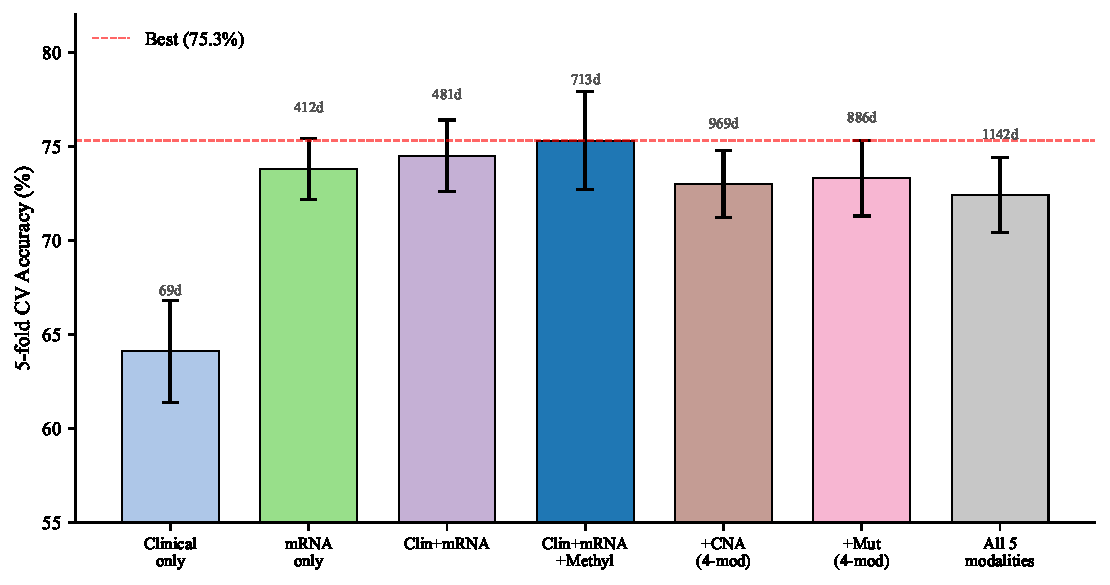
\includegraphics[width=0.9\linewidth]{figures/fig1_modality_ablation.pdf}
\caption{Modality combination ablation, with feature dimensionality annotated above each bar. The 3-modality combination (713 dimensions) is the optimum; adding copy-number or mutation blocks lowers cross-validated accuracy by 2.3 and 2.0 points respectively despite the larger input.}
\label{fig:modality_ablation}
\end{figure}

\subsection{Model Comparison and Hyperparameter Sensitivity}
\label{sec:model_comparison}

Logistic regression with $C = 0.01$ achieved the highest 5-fold cross-validation accuracy (75.3\% $\pm$ 2.6\%) among the evaluated models (Table~\ref{tab:model_comparison}; Figure~\ref{fig:model_comparison}). Ensemble methods and Transformer architectures did not surpass the linear model in this comparison. The best Transformer variant achieved 68.5\% cross-validated accuracy.

\begin{table}[htbp]
\centering
\caption{Model comparison using five-fold cross-validation on the METABRIC training subset (n=958). Models use the selected clinical + mRNA + methylation feature set (713 dimensions), unless otherwise stated.}
\label{tab:model_comparison}
\fitcol{%
\begin{tabular}{lc}
\toprule
\textbf{Model} & \textbf{CV Accuracy (\%)} \\
\midrule
Logistic Regression ($C=0.01$) & \textbf{75.3} \\
Logistic Regression ($C=0.1$) & 74.1 \\
Logistic Regression ($C=1.0$) & 72.9 \\
Calibrated LogReg (sigmoid) & 74.4 \\
Random Forest (300 trees) & 72.4 \\
XGBoost & 72.0 \\
LightGBM & 71.0 \\
CatBoost & 73.9 \\
Extra Trees & 71.3 \\
Soft-vote Ensemble (LR+GB+XGB) & 72.6 \\
Transformer ($d$=64, 2-layer) & 68.5 \\
Guided Transformer (LR prompt) & 74.0 \\
LR $\rightarrow$ Guided TF Cascade & 76.2 \\
\bottomrule
\end{tabular}}
\end{table}

\begin{figure}[htbp]
\centering
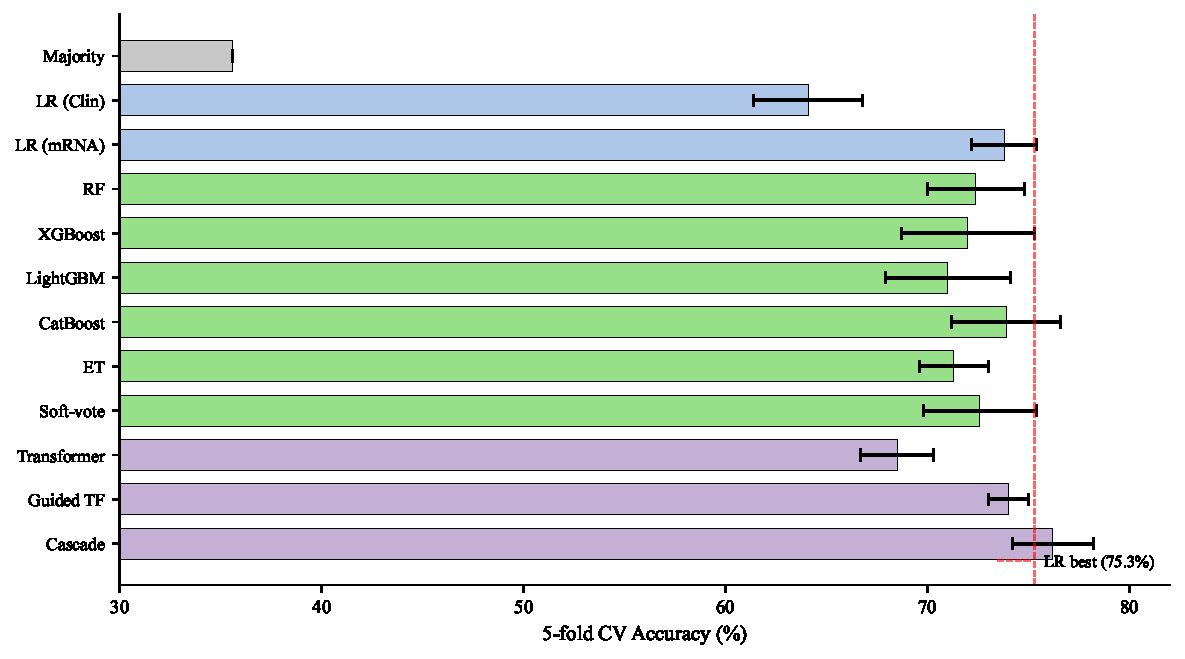
\includegraphics[width=0.85\linewidth]{figures/fig5_model_comparison.pdf}
\caption{Five-fold cross-validation model comparison on the selected METABRIC feature set.}
\label{fig:model_comparison}
\end{figure}

The cascade approach (LogReg $\rightarrow$ Guided Transformer) achieved a CV accuracy of 76.2\%, compared with 75.3\% for logistic regression alone. This 0.9-point difference was within the standard deviation of both estimates. On TCGA-BRCA, the 412-gene logistic-regression reference reached 73.8\%, whereas the unguided Transformer reached 66.1\% (Table~\ref{tab:route_a}).

\subsection{Feature Selection Identifies a Reduced Gene Set}
\label{sec:feature_selection}

ANOVA-based feature selection showed that mRNA-only cross-validated accuracy plateaued at approximately 200 genes (74.5\%). The top discriminating genes included \textit{ACOT4} ($F$=130.8), \textit{A2ML1} ($F$=102.0), and \textit{ABAT} ($F$=98.5). With clinical and methylation features, 200 mRNA genes achieved 75.5\% cross-validated accuracy, similar to the full 412-gene panel (Supplementary Table S3).

\subsection{Internal Validation Confirms Robust Performance}
\label{sec:internal}

On the held-out METABRIC test set (n=206), the 3-modality logistic regression achieved 73.8\% accuracy and 0.683 macro F1-score (Table~\ref{tab:internal_per_class}). The model showed strong performance for Luminal A (F1=0.768), Luminal B (F1=0.796), and HER2-enriched (F1=0.755) subtypes, with lower performance for Normal-like (F1=0.417) which had the smallest sample size (n=16).

\begin{table}[htbp]
\centering
\caption{Per-class classification metrics on the METABRIC test set (n=206).}
\label{tab:internal_per_class}
\fitcol{%
\begin{tabular}{lcccc}
\toprule
\textbf{Subtype} & \textbf{Precision} & \textbf{Recall} & \textbf{F1-score} & \textbf{Support} \\
\midrule
Luminal A & 0.700 & 0.851 & 0.768 & 74 \\
Luminal B & 0.812 & 0.780 & 0.796 & 50 \\
HER2-enriched & 0.741 & 0.769 & 0.755 & 26 \\
Claudin-low & 0.733 & 0.579 & 0.647 & 19 \\
Basal-like & 0.778 & 0.667 & 0.718 & 21 \\
Normal-like & 0.625 & 0.312 & 0.417 & 16 \\
\midrule
\textbf{Macro avg} & \textbf{0.732} & \textbf{0.660} & \textbf{0.683} & 206 \\
Weighted avg & 0.738 & 0.738 & 0.730 & 206 \\
\bottomrule
\end{tabular}}
\end{table}

Confusion analysis (Figure~\ref{fig:confusion}) revealed that Luminal A/Luminal B misclassification is the primary error source: 9.5\% of Luminal A samples were predicted as Luminal B, and 22.0\% of Luminal B samples were predicted as Luminal A. This reflects the biological similarity between these two subtypes, which share ER-positive status and differ primarily in proliferation rate \cite{prat2014research}. The largest single error rate is on Normal-like, 62.5\% of which is predicted as Luminal A (recall 0.312); with only 16 test samples this estimate is correspondingly imprecise.

\begin{figure}[htbp]
\centering
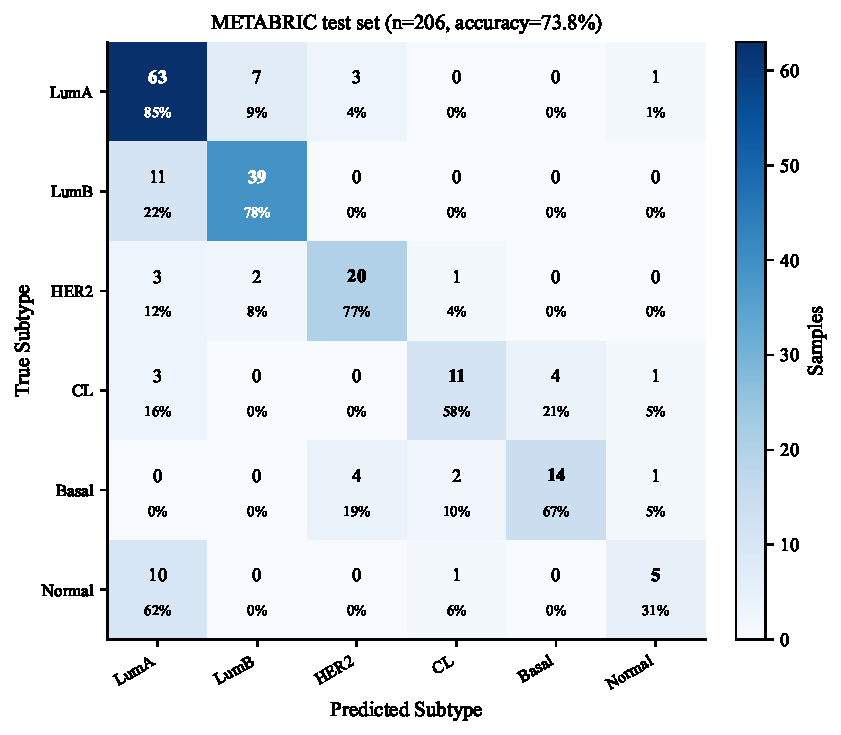
\includegraphics[width=0.85\linewidth]{figures/fig2_confusion_metabric.pdf}
\caption{Confusion matrix for the six-class PAM50 prediction task on the held-out METABRIC test set (n=206) for the 3-modality logistic regression (Clinical$+$mRNA$+$Methylation, 713 dimensions; accuracy 73.8\%). Cell values are predicted counts with row percentages. Luminal A/Luminal B confusion dominates the error budget.}
\label{fig:confusion}
\end{figure}

\subsection{External Validation Across Distinct Cohorts}
\label{sec:external}

The 412-gene mRNA-only model with within-platform rank normalization achieved 73.8\% accuracy on TCGA-BRCA (n=987, Figure~\ref{fig:tcga}), similar to its 73.8\% accuracy on the held-out METABRIC test set. The default external evaluation is restricted to mRNA because TCGA's clinical schema is not mappable to METABRIC's in full: it records no Nottingham Prognostic Index or IntClust assignment, has no equivalent of the three-gene classifier or cohort field, and uses different therapy, cellularity and histology vocabularies; only sixteen of the 69 clinical dimensions have a defensible counterpart. A reduced clinical block and a TCGA methylation block can both be constituted, however, and Section~\ref{sec:external_multimodal} uses them to test whether the internal multimodal advantage transfers. The survival C-index was 0.577 ($p = 0.047$, log-rank test).

\begin{table}[htbp]
\centering
\caption{Per-class classification metrics on TCGA-BRCA external validation (n=987, 5 subtypes).}
\label{tab:tcga_per_class}
\fitcol{%
\begin{tabular}{lcccc}
\toprule
\textbf{Subtype} & \textbf{Precision} & \textbf{Recall} & \textbf{F1-score} & \textbf{Support} \\
\midrule
Luminal A & 0.904 & 0.749 & 0.819 & 502 \\
Luminal B & 0.600 & 0.709 & 0.650 & 199 \\
HER2-enriched & 0.667 & 0.846 & 0.746 & 78 \\
Basal-like & 0.978 & 0.762 & 0.856 & 172 \\
Normal-like & 0.500 & 0.389 & 0.438 & 36 \\
\bottomrule
\end{tabular}}
\end{table}

\begin{table}[htbp]
\centering
\caption{Raw confusion matrix for TCGA-BRCA external validation (n=987), rows true and columns predicted. Claudin-low appears as a predicted column but not as a true row because TCGA-BRCA carries no claudin-low annotations: all 75 samples the model places there are necessarily errors. Basal-like $\rightarrow$ claudin-low (38 samples) is the single largest off-diagonal block.}
\label{tab:tcga_confusion}
\fitcol{%
\begin{tabular}{lcccccc}
\toprule
\textbf{True $\backslash$ Pred} & \textbf{LumA} & \textbf{LumB} & \textbf{Her2} & \textbf{CL} & \textbf{Basal} & \textbf{Normal} \\
\midrule
Luminal A & \textbf{376} & 87 & 10 & 15 & 0 & 14 \\
Luminal B & 37 & \textbf{141} & 18 & 3 & 0 & 0 \\
HER2-enriched & 2 & 5 & \textbf{66} & 3 & 2 & 0 \\
Basal-like & 0 & 0 & 3 & 38 & \textbf{131} & 0 \\
Normal-like & 1 & 2 & 2 & 16 & 1 & \textbf{14} \\
\midrule
\textbf{Predicted total} & 416 & 235 & 99 & \textbf{75} & 134 & 28 \\
\bottomrule
\end{tabular}}
\end{table}

Macro F1 depends on the set of classes included in the average. We report it over the six-class label space used for training. METABRIC contains all six classes and has macro F1 0.683. TCGA contains five PAM50 classes, so claudin-low contributes an F1 of zero and the six-class average is 0.585. Averaging the same predictions over the five PAM50 classes gives macro F1 \textbf{0.702}. This 0.117 difference is caused by the metric's class set; it does not represent a change in predictions. Separately, the classifier predicted claudin-low for 75 TCGA samples (7.6\%). Those predictions were errors and included 22.1\% of basal-like and 44.4\% of Normal-like samples. TCGA also had a higher Luminal A prevalence than METABRIC (50.9\% versus 36\%) and only 36 Normal-like samples, of which 14 were correctly classified.

\begin{figure}[htbp]
\centering
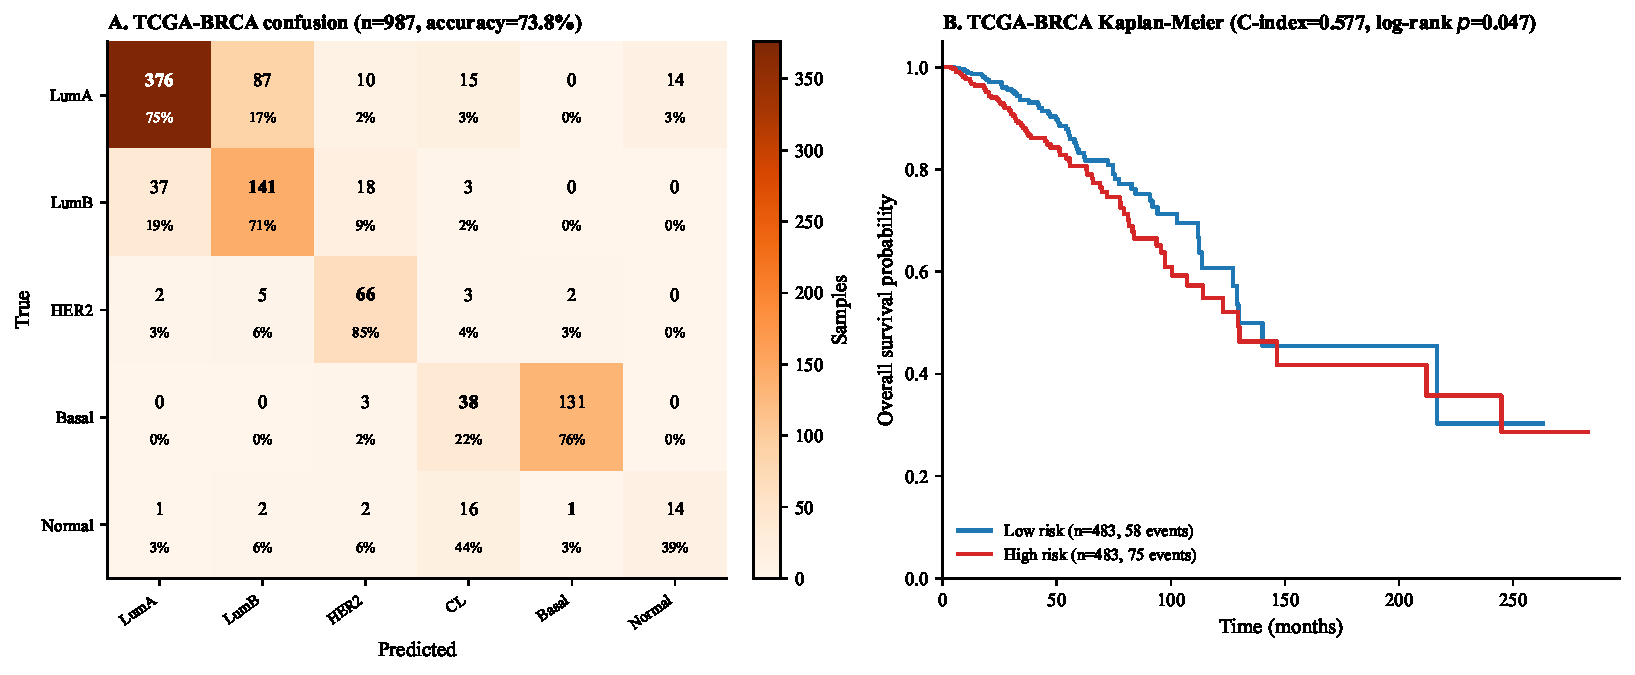
\includegraphics[width=0.8\linewidth]{figures/fig3_tcga_results.pdf}
\caption{External validation on TCGA-BRCA (n=987). The within-platform rank-normalized mRNA model reaches 73.8\% accuracy and a survival C-index of 0.577 ($p$=0.047).}
\label{fig:tcga}
\end{figure}

\subsection{The Multimodal Advantage Does Not Survive External Validation}
\label{sec:external_multimodal}

The three-modality result in Section~\ref{sec:modality} was established on a single cohort. To test whether it generalizes, we constructed a reduced space that METABRIC and TCGA-BRCA both carry and re-ran the modality ablation inside it. Three layers were harmonized. mRNA uses the same 412-gene panel, matched by symbol on both platforms (all 412 present; 10 are invariant on TCGA and were assigned the neutral score). Methylation uses the 232-gene METABRIC panel, which is already gene-level because the METABRIC preprocessing reduced probes to genes by variance; the corresponding TCGA-BRCA HM450 gene-level values were retrieved from cBioPortal, and 209 of the 232 genes carry measurements (23 are absent from the array). Clinical uses the 10 fields present in both schemas: age, pathologic stage, ER, PR, and HER2 status, and menopausal state. Every continuous feature was rank-transformed to normal scores \emph{within its own cohort}, a label-free operation, so no target labels were used at any point. Requiring all three layers plus an annotated subtype leaves 694 TCGA-BRCA patients across the five PAM50 classes; claudin-low is absent, as in the n=987 cohort.

Table~\ref{tab:multimodal_external} reports the ablation in this space, and the pattern reverses. Adding methylation produces no cross-validated gain on METABRIC (72.91\% for mRNA alone versus 72.91\% for mRNA plus methylation) and lowers TCGA accuracy by 1.9 points, from 80.55\% to 78.67\%. Adding the harmonized clinical block raises METABRIC cross-validated accuracy by 0.5 points and the held-out METABRIC test score by 2.4 points, but moves TCGA accuracy by only 0.3 points in the unrestricted setting and $-0.15$ points under the five-class restriction. No multimodal configuration differs significantly from mRNA alone (paired McNemar, $p = 0.13$ to $1.00$), and the confidence intervals in Table~\ref{tab:multimodal_ci} overlap almost completely.

\begin{table}[htbp]
\centering
\caption{Modality ablation in the harmonized three-layer space shared by METABRIC and TCGA-BRCA. CV is five-fold cross-validated accuracy on pooled METABRIC train+val (n=1{,}163). TCGA accuracy is on n=694 patients annotated with one of the five PAM50 classes present in that cohort. The McNemar column is a paired test against mRNA alone. The final row is the original 713-dimension model, shown for reference: its clinical block includes METABRIC-specific fields and has no external counterpart.}
\label{tab:multimodal_external}
\fitcol{%
\begin{tabular}{lcccccc}
\toprule
\textbf{Configuration} & \textbf{Dims} & \textbf{METABRIC CV} & \textbf{METABRIC test} & \textbf{TCGA} & \textbf{TCGA macro F1} & \textbf{$p$} \\
\midrule
mRNA                 & 412 & 72.91 & 72.82 & \textbf{80.55} & 0.768 & --- \\
mRNA + clinical      & 422 & 73.43 & \textbf{75.24} & 80.40 & \textbf{0.774} & 1.00 \\
mRNA + methylation   & 644 & 72.91 & 72.33 & 78.67 & 0.747 & 0.13 \\
clinical + mRNA + methylation & 654 & 73.17 & 74.76 & 79.11 & 0.760 & 0.30 \\
\midrule
\emph{original flagship} & \emph{713} & \emph{75.92} & \emph{73.79} & \emph{n/a} & \emph{n/a} & \emph{---} \\
\bottomrule
\end{tabular}}
\end{table}

\begin{table}[htbp]
\centering
\caption{Bootstrap 95\% confidence intervals (2{,}000 patient resamples) for the harmonized configurations on TCGA-BRCA (n=694). Restricted accuracy is computed over the five PAM50 classes present; unrestricted accuracy scores all six candidate labels.}
\label{tab:multimodal_ci}
\fitcol{%
\begin{tabular}{lcc}
\toprule
\textbf{Configuration} & \textbf{Accuracy (restricted)} & \textbf{Macro F1 (restricted)} \\
\midrule
mRNA                 & 0.775--0.834 & 0.725--0.808 \\
mRNA + clinical      & 0.774--0.833 & 0.731--0.814 \\
mRNA + methylation   & 0.755--0.817 & 0.703--0.786 \\
clinical + mRNA + methylation & 0.759--0.820 & 0.717--0.798 \\
\bottomrule
\end{tabular}}
\end{table}

\begin{figure}[htbp]
\centering
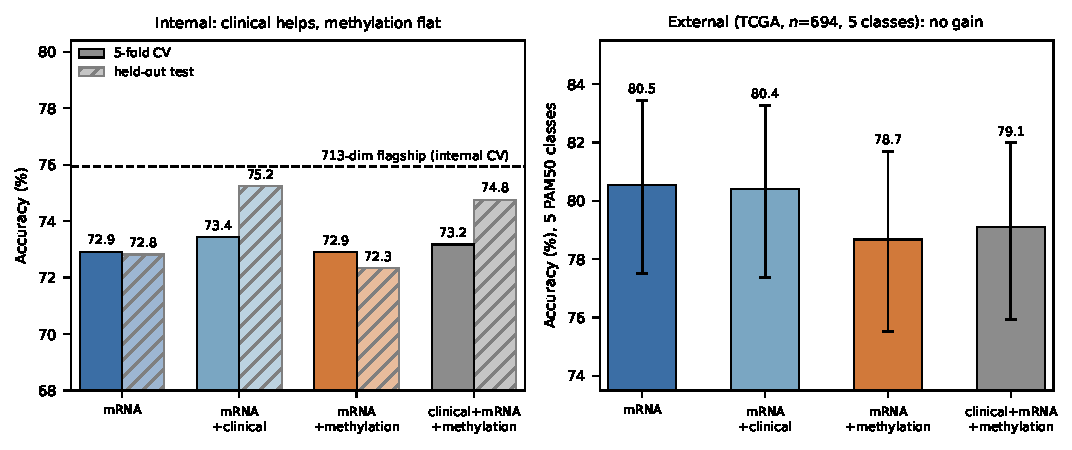
\includegraphics[width=0.95\linewidth]{figures/figJ_multimodal_external.pdf}
\caption{The multimodal advantage does not transfer. Panel A: internal cross-validated and held-out METABRIC accuracy for each configuration, with the original 713-dimension flagship as a reference line. Panel B: TCGA-BRCA accuracy over the five PAM50 classes present (n=694) with bootstrap 95\% confidence intervals. Every configuration's interval overlaps the mRNA-only interval; the harmonized clinical block helps internally and is negligible externally.}
\label{fig:multimodal_external}
\end{figure}

The two internal blocks move in opposite directions from their external counterparts. On METABRIC the harmonized tri-modal model reaches 73.17\% cross-validated accuracy, while the original 713-dimension flagship reaches 75.92\%. That 2.75-point gap is attributable to the 59 clinical dimensions that exist only in METABRIC (NPI, GRADE, INTCLUST membership, THREEGENE proliferation class, and cohort indicator); those fields are not available in the target cohort, so the model that performs best internally is precisely the one that cannot be transported. Conversely, the harmonized model's higher absolute TCGA accuracy (80.55\% versus the published 73.76\%) reflects the label-space restriction, not better prediction: under the five-class restriction the 64 samples the mRNA model sends to the absent claudin-low column are reallocated to in-space classes, which is the same evaluation-rule change quantified in Section~\ref{sec:labelspace}.

We report this as a negative result about modality fusion, not as a failure of the pipeline. The consistent finding is that additional modalities and additional architectural capacity raise internal cross-validated scores while leaving or worsening external accuracy. The one intervention that improved external performance was correcting the label space, not adding features.

\subsection{Label-Space Reconciliation Changes Cross-Cohort Evaluation}
\label{sec:labelspace}

Uncorrected accuracy on TCGA-BRCA (73.76\%) was similar to that on the METABRIC test set (73.8\%), whereas accuracy on GSE21653 was lower (63.16\%). These observations do not support a general claim that label-space mismatch explains every cross-cohort accuracy difference. However, both external cohorts use PAM50 annotations, whose five intrinsic subtypes exclude claudin-low, whereas the METABRIC classifier was trained on six classes. We therefore measured how explicitly reconciling the label space changes the reported metrics, separately from prior correction, without attributing all residual differences to annotation mismatch.

Predictions assigned to a class excluded by the target's annotation standard are necessarily counted as errors under that standard. In TCGA, the model assigned 75 samples (7.6\%) to claudin-low. These predictions included 22.1\% of basal-like and 44.4\% of Normal-like samples. The resulting recall changes depend on which classes the model confuses with claudin-low.

\subsection{Effect of Label-Space Reconciliation and Prior Correction}

Table~\ref{tab:labelspace} decomposes the correction on both external cohorts. Restricting the output space to the five PAM50 classes and renormalising (mask\_only) already moves TCGA-BRCA from 73.76\% to 79.74\% and GSE21653 from 63.16\% to 68.42\%. Adding EM prior correction over the reconciled space (em\_pam50) gives \textbf{80.65\%} on TCGA-BRCA and \textbf{74.06\%} on GSE21653, with macro F1 rising from 0.585 to 0.737 and from 0.504 to 0.683 respectively. On GSE21653 this is a 10.90-point increase relative to the uncorrected estimate. Because the procedure changes both the allowed label set and the estimated class priors, this increase should be interpreted as an evaluation and post-processing effect, not a gain in learned discrimination.

One detail in the table deserves emphasis rather than omission: EM prior correction trades macro F1 for accuracy. On TCGA-BRCA, mask\_only already reaches macro F1 0.757, and the prior correction lowers it to 0.737 while raising accuracy from 79.74\% to 80.65\%. The correction shifts mass toward the dominant class, which can improve overall accuracy at the expense of rarer classes. This is consistent with prior matching and motivates reporting both metrics. The choice between the two rows is therefore a decision about which error matters clinically, not a strictly dominated one; the label-space restriction is unambiguously beneficial (macro F1 0.585 $\rightarrow$ 0.757), while the additional prior correction is a trade-off that a deployment could reasonably decline. The multiclass Brier score, however, improves monotonically along base $\rightarrow$ mask\_only $\rightarrow$ em\_pam50 on both cohorts (TCGA: 0.376 $\rightarrow$ 0.291 $\rightarrow$ 0.275; GSE21653: 0.492 $\rightarrow$ 0.427 $\rightarrow$ 0.378), so the correction produces better probability estimates in a proper-scoring sense rather than merely relabelling the argmax (Supplementary Section~S3).

\begin{table}[htbp]
\centering
\caption{Decomposition of the cross-cohort correction. Within each cohort, all rows share one classifier and feature set, using logistic regression ($C$=0.01) and within-platform rank normalization. TCGA-BRCA uses 412 genes; GSE21653 uses the 369 genes mapped to GPL570, with a source model refitted on those genes. Rows differ only in label-space handling. \textbf{mask\_only} uses the annotation-standard fact that claudin-low is not a PAM50 subtype; \textbf{em\_pam50} adds EM prior correction on the reconciled space; \textbf{em\_full} runs EM without label-space knowledge. Neither the mask nor any row uses target labels.}
\label{tab:labelspace}
\fitcol{%
\begin{tabular}{lcccc}
\toprule
 & \multicolumn{2}{c}{\textbf{TCGA-BRCA (n=987)}} & \multicolumn{2}{c}{\textbf{GSE21653 (n=266)}} \\
\cmidrule(lr){2-3}\cmidrule(lr){4-5}
\textbf{Estimator} & Acc (\%) & Macro F1 & Acc (\%) & Macro F1 \\
\midrule
base (no reconciliation) & 73.76 & 0.585 & 63.16 & 0.504 \\
mask\_only & 79.74 & 0.757 & 68.42 & 0.626 \\
em\_pam50 & \textbf{80.65} & \textbf{0.737} & \textbf{74.06} & \textbf{0.683} \\
em\_full (no mask) & 75.99 & 0.586 & 68.42 & 0.541 \\
\bottomrule
\end{tabular}}
\end{table}

Figure~\ref{fig:cross_platform} compares one mRNA-only estimator across three cohorts. The estimator uses 412 genes, $C$=0.01, and within-platform rank normalization, with no retraining. Accuracy was 74.6\% on METABRIC validation, 73.8\% on the METABRIC test set, and 73.8\% on TCGA-BRCA. Six-class macro F1 was 0.720, 0.706, and 0.585, respectively. For TCGA, averaging over the five PAM50 classes instead gives 0.702. Thus, the macro-F1 difference depends in part on the class set used for scoring; these metrics alone do not establish unchanged model discrimination.

\begin{figure}[htbp]
\centering
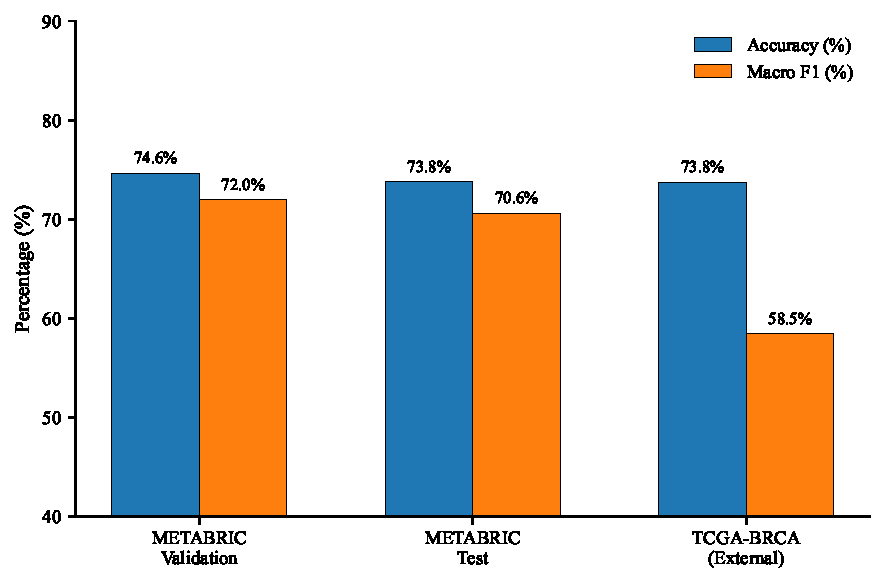
\includegraphics[width=0.7\linewidth]{figures/fig6_cross_platform.pdf}
\caption{Accuracy and macro F1 for the same mRNA-only estimator across METABRIC validation, METABRIC test, and TCGA-BRCA. TCGA accuracy is similar to the internal estimates, while the six-class macro F1 is affected by the absent claudin-low class.}
\label{fig:cross_platform}
\end{figure}

\subsection{Unlabelled Predictions Did Not Recover the Label Space}

We tested whether the absent class could be detected without annotation-space information. Unconstrained EM and two detector procedures did not reliably identify it in the tested settings. \emph{The detection-F1 figures quoted in this and the following two subsections come from the original scoring function, which returns zero when a detector correctly predicts the empty set; every cohort with no absent class was therefore scored as a total failure irrespective of the detector's answer. Section~\ref{sec:detector_v2} re-scores the same simulation under the standard empty-set convention and should be read as the reference for detector ranking.}

Running the same EM procedure without the mask (em\_full), using the same classifier and unlabelled target predictions, leaves claudin-low with an estimated prior of \textbf{0.0751} on TCGA-BRCA and 0.0719 on GSE21653, against a true prevalence of exactly 0. EM has no signal with which to push that mass to zero: a class that is absent from the label space still receives probabilistic predictions, and those predictions are indistinguishable from genuine low-confidence assignments to a rare class. The result is that em\_full recovers only 2.2 of the 6.9 available points on TCGA-BRCA and leaves macro F1 essentially unchanged (0.585 $\rightarrow$ 0.586), whereas the masked version, given one bit of annotation knowledge, recovers 6.9 points. We stress that the two runs differ in nothing else.

In this experiment, the predicted marginal was compatible with both an absent class and a rare class. These results do not prove that no function of unlabeled predictions can distinguish those cases under any model. They show that the annotation-space fact was not recovered by the tested EM procedure and detectors.

\subsection{A Calibrated Detector Fails to Recover It}

We did not accept that conclusion without testing the obvious workaround: detect the absent class geometrically. On the probability simplex, a truly absent class should show a deficit of observed mass relative to its source-expected mass, and we built the ratio statistic described in Section~\ref{sec:methods_detector} to exploit exactly that. We calibrated the threshold on null data, consisting of cohorts with no absent class, at level $\alpha = 0.05$, so that a clean cohort is flagged at most 5\% of the time. This calibration is what makes the test fair; an uncalibrated threshold would flag absence everywhere.

The detector fails. The null-calibrated threshold is $\tau^* = 1.0349$, against a null maximum ratio with median 1.0184 and maximum 1.0493. Because the null distribution of the maximum ratio almost reaches the calibrated threshold, the statistic has almost no power: on the calibration set precision is 0.257 and recall 0.643 (F1 0.367). In the controlled simulation its mean detection F1 is \textbf{0.047} against \textbf{0.549} for EM. Its performance depended on the baseline. Against the uncorrected model it helped on average (mean $+3.34$ points over 30 cells) but was not reliable. Its worst cell is $-2.77$ points, on a cohort with no absent class (73.98\% $\rightarrow$ 71.22\%), precisely because $\tau^*$ flags absent classes that are not there. Against EM, the procedure it was built to replace, it does not help at all: it wins outright in 11 cells, loses in 9, ties in 10, and its mean gain is \textbf{$-0.37$ points}.

We also tested a generative model-selection detector described in Section~\ref{sec:methods_lrt}. It fits the target sample as a Gaussian mixture with source-derived components and selects the label space that minimises BIC over subsets with zero, one, or two absent classes. The complexity penalty replaces a hand-set threshold. On 30 null cohorts with every class present, it selects a non-empty absent set in \textbf{27 of 30 runs (90\%)}, and in 23 of those it claims \emph{two} absent classes. Its mean detection F1 in simulation is 0.209 against 0.549 for EM, and it loses to EM on accuracy in \textbf{all 30 of 30} cells, by a mean of 17.6 points. A BIC-style penalty is not sufficient to make an absent class identifiable.

Both detector procedures produced negative results in the tested settings. The geometric statistic had low detection performance, while the model-selection procedure produced false positives on clean cohorts. These findings support specifying the target label space from cohort documentation rather than relying on the tested detectors.

\subsection{A Corrected Metric Reverses the Detector Ranking}
\label{sec:detector_v2}

The comparison above used a scoring function that returns 0.0 whenever a detector correctly predicts the empty set, because the F1 numerator and denominator both vanish; every cohort with no absent class was therefore scored as a total failure regardless of whether the detector was right. Under the standard empty-set convention the comparison changes substantially, so we re-ran the simulation scoring each cell with micro precision, recall, and exact-set match, over 20 seeds per cell, six absent sets, three covariate-shift levels, and with and without a Dirichlet prior shift, giving 720 evaluated cohorts. Raw detected and true sets were written to disk so the scoring can be re-examined without re-running the simulation.

Table~\ref{tab:detector_v2} gives the pooled result. The uncalibrated EM rule that the earlier analysis reported as failing is in fact the strongest of the six on F1 and exact-set match: F1 0.786 and exact-set-match 0.550, both above every calibrated alternative. The multiplicity-controlled replacement, which resamples source validation predictions to build a null and applies Benjamini--Hochberg at $\alpha = 0.05$, is markedly more aggressive: precision falls to 0.577 and it flags a non-empty absent set on 73 of the 120 clean cohorts. The probability-frequency rule flags 87 of 120. Importance weighting the null by a discriminator-estimated density ratio reduces clean-cohort errors to 56 of 120 but also halves recall, buying specificity at a real cost in power. Declaring a class absent because the model never predicts it attains perfect precision and an exact-match rate of 0.167 by predicting nothing, which is the degenerate solution the empty-set convention exposes rather than rewards.

\begin{table}[htbp]
\centering
\caption{Absent-class detectors scored with the standard empty-set convention (20 seeds $\times$ 6 absent sets $\times$ 3 covariate-shift levels $\times$ 2 prior-shift settings $=$ 720 cohorts). Null false positives count cohorts with no absent class on which the detector returned a non-empty set. The na\"ive exact-match rate of 0.167 is the fraction of settings in which nothing was in fact absent.}
\label{tab:detector_v2}
\fitcol{%
\begin{tabular}{lccccc}
\toprule
\textbf{Detector} & \textbf{Micro P} & \textbf{Micro R} & \textbf{F1} & \textbf{Exact} & \textbf{Null FP} \\
\midrule
Uncalibrated EM (\emph{em\_orig}) & \textbf{0.920} & 0.685 & \textbf{0.786} & \textbf{0.550} & 17/120 \\
Calibrated EM (\emph{em\_cal}) & 0.577 & \textbf{0.876} & 0.696 & 0.362 & 73/120 \\
Importance-weighted EM (\emph{em\_cal\_iw}) & 0.540 & 0.544 & 0.542 & 0.242 & 56/120 \\
Probability frequency (\emph{pfreq}) & 0.548 & 0.902 & 0.682 & 0.372 & 87/120 \\
Geometric coherence (\emph{geo}) & 0.467 & 0.154 & 0.232 & 0.193 & 27/120 \\
Never predicted (\emph{naive}) & 1.000 & 0.006 & 0.012 & 0.167 & \textbf{0/120} \\
\bottomrule
\end{tabular}}
\end{table}

The pooled figures conceal the structure that matters: detection degrades with covariate shift and fails differently under prior shift. Restricting to cohorts with a truly absent class, the uncalibrated rule's mean F1 is 0.995 with no covariate shift and no prior shift, falling to 0.543 at the highest covariate-shift level with prior shift present. The calibrated detectors lose control of the clean-cohort error rate when prior shift is present. With no prior shift the uncalibrated rule flags none of the 20 clean cohorts at any covariate-shift level (0/20), while \emph{em\_cal} flags 3, 2, and 11 of 20 and \emph{pfreq} flags 11, 9, and 7 of 20 as the covariate shift rises from 0.0 to 0.8. Under prior shift the uncalibrated rule still flags only 9, 3, and 5 of 20, but \emph{pfreq} flags all 20 clean cohorts at every covariate-shift level and \emph{em\_cal} flags 20, 18, and 19 of 20. No detector is simultaneously high-recall and low-false-positive across both shift axes.

The practical conclusion is unchanged but now rests on corrected measurement rather than a metric artefact. Absence of a class is not identifiable from unlabelled predictions by any tested procedure once covariate and prior shift are both present, and the apparent failure of the original rule was overstated: it is the strongest detector tested on F1 and exact-set match, and its calibrated replacements trade that strength for clean-cohort false positives.

\subsection{Separating Label-Space Mismatch from Prior Shift}

Because the real cohorts change both prevalence and label space simultaneously, we simulated the two factors independently: label-space mismatch $n_{\text{absent}} \in \{0,1,2\}$, covariate shift, and prior shift, 20 seeds per cell, $n_{\text{target}} = 1000$ (Section~\ref{sec:methods_sim}). The separation is clean. With \emph{no} prior shift the correction is worth $-0.4$ to $+3.2$ points, straddling zero and growing only with the number of absent classes: with no prior shift the label-space term alone contributes roughly $+0.7$ to $+3.2$ points. With prior shift the correction is worth $+5.9$ to $+7.9$ points in every cell. The mechanism is that label-space mismatch creates \emph{apparent} prior shift on the remaining classes. EM can only redistribute mass within the supplied label space, so the two effects can interact in real cohorts.

The simulation also reproduces the identifiability failure at scale: the oracle-mask column matches the detected column only when the mask is supplied, and the unguided detector's accuracy tracks the uncorrected baseline once the absent class is rare.

\subsection{Claudin-Low Is the Mildest Case, Not a Representative One}
\label{sec:absence_generality}

The real-cohort analysis turns on a single absent class, claudin-low, which is also the rarest in the source prior (9.5\% of METABRIC). A reader may reasonably ask whether the effect is representative of label-space mismatch or merely its smallest instance, so we swept the absence pattern over which class is missing and how it is missing, holding everything else fixed (Supplementary Section~S5).

Severity is governed by the absent class's \emph{prior mass}, not by its identity. Dropping \textbf{Luminal A} -- the commonest class, at 35.7\% of the source -- costs 11.33 points of naive accuracy, all recoverable ($74.67\% \rightarrow 86.00\%$); dropping claudin-low costs 1.74 points. The class we study is thus the mildest instance, by roughly a factor of six.

More consequential is \emph{how} the class goes missing. Annotation disagreement rarely takes the form of a class disappearing; far more often one class is recorded under a neighbour's label. A Luminal B relabelled as Luminal A -- two subtypes sharing receptor status and differing mainly in proliferation -- leaves naive accuracy at a reassuring 79.43\% while concealing a recoverable loss of \textbf{12.0 points}, the largest in the sweep, and the label-free detector recovers it only partially (detection F1 0.767). Partial absence defeats detection outright for the classes that matter most: when prevalence is scaled to $\tau_{\text{ratio}}$ of source rather than zeroed, detection F1 is \textbf{0.000} for Luminal A and \textbf{0.067} for Luminal B, against 0.967 for claudin-low. The identifiability failure is therefore worst exactly where the consequences are largest, which strengthens the practical recommendation: the target's allowed labels should be read off the cohort documentation, not inferred from predictions.

\subsection{Stability of the Correction}

The correction does not depend on how the target is partitioned. Splitting TCGA-BRCA in half and applying the procedure transductively within each half gives 80.97\% and 80.12\%, a spread of 0.85 points compared with the recovered gain of 6.89. A paired bootstrap over target samples ($n_{\text{iter}} = 2000$) gives a mean gain of \textbf{+6.88 points}, 95\% CI \textbf{[+4.96, +8.81]}, with $P(\text{gain} > 0) = 1.0$. The gain is therefore not an artifact of a favourable partition or of a few influential samples.

\subsection{A Five-Class Training Baseline Reaches the Same Accuracy on TCGA}
\label{sec:fiveclass}

The estimator above reconciles the label space at evaluation time. A simpler
alternative is to train on five classes directly. We built both variants -- dropping
the 91 claudin-low training samples (n=867), and relabelling them as Basal-like
(n=958) -- on the same features and hyperparameters, and compared them with the
six-class estimator on the identical external cohorts (Supplementary
Table~S2).

On TCGA-BRCA the five-class \emph{drop} model reaches 80.04\% against 80.65\% for the
six-class estimator with EM correction, and a paired McNemar test does not separate
them ($p = 0.50$); it also attains the highest macro F1 of any configuration (0.774).
On GSE21653 the six-class estimator with EM correction is significantly better
(74.06\% against 69.55\%, $p = 0.003$). The difference is the prior correction, not the
label space: on GSE21653 the label-space step alone gives 68.42\%, statistically
indistinguishable from the five-class model, and EM then adds a further 5.6 points by
re-estimating the target priors in a basal-enriched cohort.

The interpretation we draw is that label-space \emph{reconciliation} accounts for most
of the recovered accuracy on TCGA, whereas prior correction contributes materially only
when the target composition departs from the source. This does not change the reported
result -- 73.76\% remains an artefact of evaluating a six-class model against a
five-class standard -- but it does mean that a five-class training run is a legitimate
design when the target label space is known in advance, and we say so rather than
claiming the reconciliation procedure is uniquely necessary.

\begin{figure}[htbp]
\centering
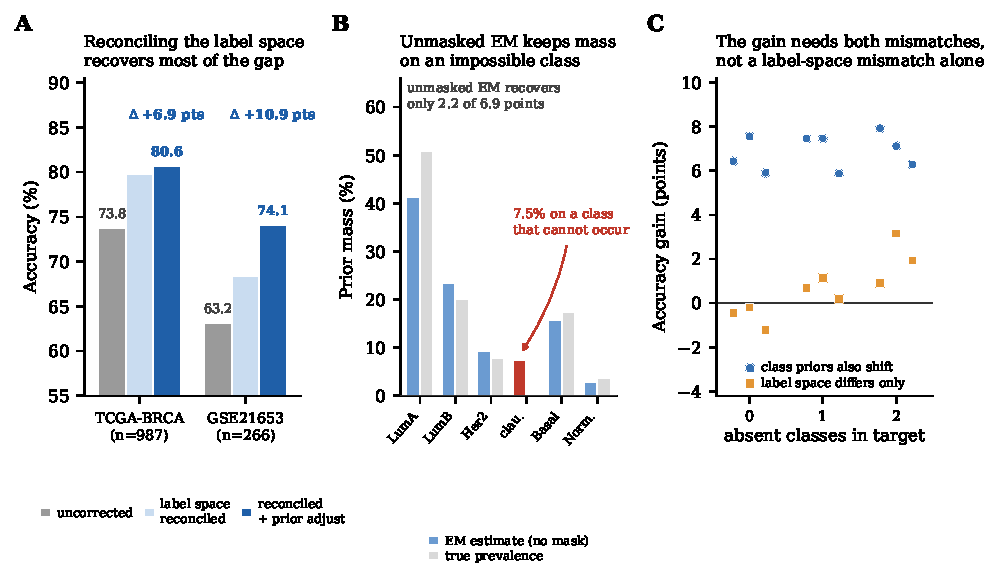
\includegraphics[width=0.85\linewidth]{figures/figH_label_shift.pdf}
\caption{Label-space reconciliation and prior correction. \textbf{(A)} Accuracy before and after label-space reconciliation on TCGA-BRCA and GSE21653, showing the mask-only and EM-corrected stages separately. \textbf{(B)} The identifiability failure: unconstrained EM retains substantial prior mass on claudin-low, whose true prevalence in both cohorts is zero, and recovers only a fraction of the available gain. \textbf{(C)} Controlled simulation separating label-space mismatch from prior shift; the correction is near zero without prior shift and consistently large with it.}
\label{fig:label_shift}
\end{figure}

\subsection{Survival Analysis Validates Prognostic Stratification}
\label{sec:survival}

Cox proportional hazards regression on the METABRIC validation + test sets (n=411, 267 death events, 65\% event rate) showed that predicted subtype probabilities carry statistically significant prognostic information ($p = 0.0008$), though the overall C-Index of 0.598 is modest and comparable to other single-feature prognostic models in breast cancer \cite{prat2014research}. Time-dependent C-Indices were 0.651 (3-year), 0.622 (5-year), and 0.610 (10-year).

\begin{table}[htbp]
\centering
\caption{Cox regression hazard ratios for predicted subtypes (Luminal A = reference) on METABRIC (n=411).}
\label{tab:cox}
\fitcol{%
\begin{tabular}{lccc}
\toprule
\textbf{Predicted Subtype} & \textbf{HR} & \textbf{95\% CI} & \textbf{p-value} \\
\midrule
Luminal B & 1.50 & [1.14, 1.97] & $<0.005$ \\
HER2-enriched & 1.43 & [1.08, 1.89] & 0.01 \\
Basal-like & 1.46 & [1.07, 1.99] & 0.02 \\
Claudin-low & 0.82 & [0.58, 1.16] & 0.25 \\
Normal-like & 1.31 & [0.86, 2.00] & 0.21 \\
\bottomrule
\end{tabular}}
\end{table}

On the TCGA-BRCA cohort (n=966, 133 events), the C-Index was 0.577 ($p = 0.047$), with time-dependent C-Indices of 0.587 (3-year), 0.574 (5-year), and 0.577 (10-year). The concordant survival discrimination across both cohorts (0.598 internally, 0.577 and 0.584 externally) is modest but consistent, suggesting the risk signal generalizes across platforms despite the limited discriminative power. The risk score is a Cox model fit on METABRIC training predictions and applied unchanged to TCGA, which requires no outcome information from the validation cohort and is therefore fully reproducible from the released code. An earlier iteration of this analysis reported a C-index of 0.586 ($p = 0.013$) under a variant risk-score construction whose exact form was not retained; because that construction cannot be reconstructed from the preserved pipeline, we report the reproducible figures throughout rather than mixing the two.

\subsection{SHAP Analysis Reveals Modality Contributions}
\label{sec:shap}

SHAP interpretability analysis (Figure~\ref{fig:shap}) quantified the relative importance of each modality. Because the classifier is linear, these attributions are exact and sum to the model's output, so they can be read as the model's own decomposition of its decisions. mRNA expression contributed 63.3\%, methylation 26.7\% and clinical features 10.0\%; copy number and mutation data contributed $<$1\% each, consistent with their noise-inducing effect in the ablation. These figures describe \emph{this} fitted model on \emph{this} encoding; they are not evidence that the two weak modalities carry no biological signal, only that the present architecture and feature representation extract little from them.

The top discriminating features included ER/HER2 clinical markers and proliferation features. Leading mRNA features included \textit{ACP7}, \textit{ACTG2}, \textit{ADIRF}, and \textit{ACOT4}. These features align with established breast cancer biology and PAM50 subtype definitions.

\begin{figure}[htbp]
\centering
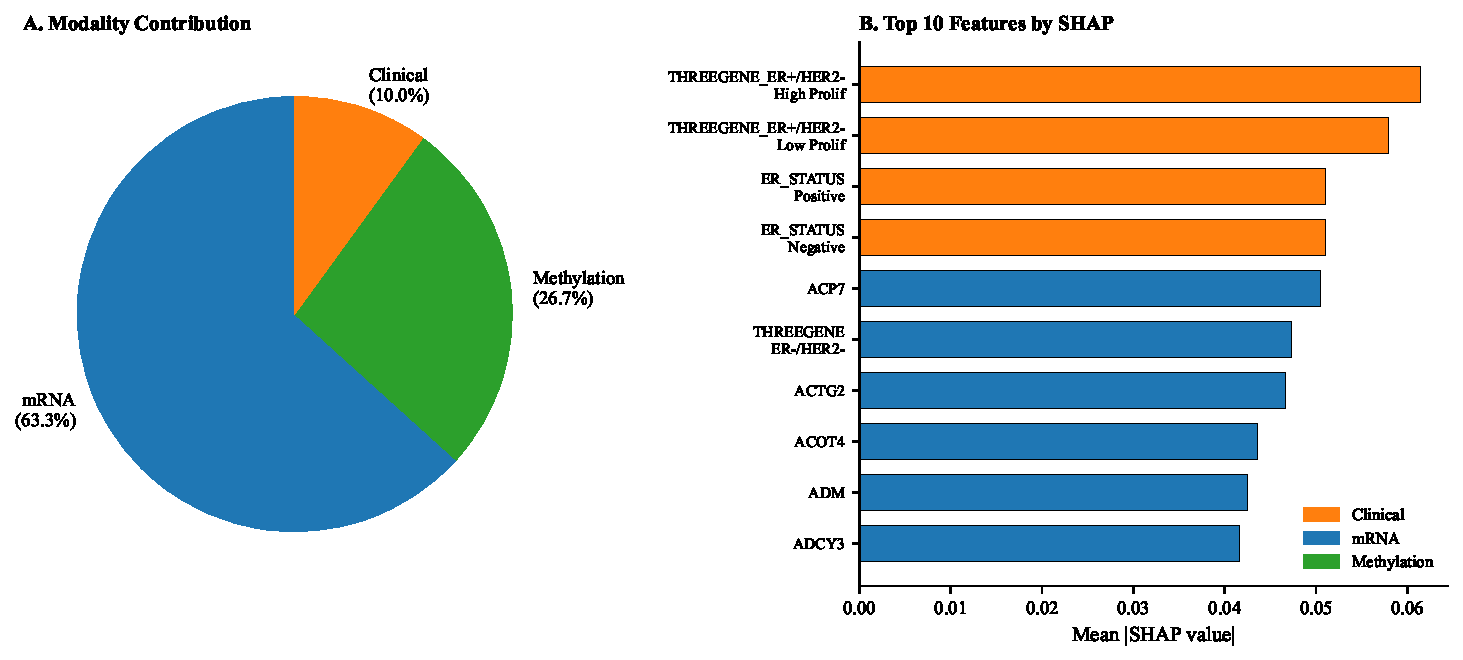
\includegraphics[width=0.8\linewidth]{figures/fig4_shap_analysis.pdf}
\caption{SHAP-based modality attribution. mRNA expression accounts for 63.3\% of model decisions, methylation 26.7\% and clinical features 10.0\%; copy-number and mutation blocks contribute under 1\% each.}
\label{fig:shap}
\end{figure}

\subsection{The Genomic Panel Outperforms Subtype Alone in Treated Subgroups}
\label{sec:route_a_treatment}

We also asked whether the 713-dimension panel adds information beyond the subtype call itself for clinically relevant stratified outcomes. We defined a 5-year outcome (death within 60 months versus survival beyond it, censored observations excluded) and evaluated within treatment subgroups, using the same 5-fold protocol and reporting AUC against a PAM50 subtype-only baseline trained on the identical splits.

A necessary caveat: METABRIC's treatment fields record whether a therapy was \emph{administered}, not whether the patient responded. There is no response variable in this dataset, so this is \emph{prognosis among treated patients}, not treatment-response prediction, and we label it as such throughout.

\begin{table}[htbp]
\centering
\caption{5-year outcome discrimination within treatment subgroups, genomic panel versus PAM50 subtype alone. These are administered-treatment cohorts, not response assessments.}
\label{tab:treatment}
\fitcol{%
\begin{tabular}{lccccc}
\toprule
\textbf{Treated subgroup} & \textbf{n} & \textbf{Events} & \textbf{AUC (panel)} & \textbf{AUC (subtype)} & \textbf{$\Delta$} \\
\midrule
Chemotherapy & 275 & 120 & 0.624 & 0.571 & $+0.053$ \\
Hormone therapy & 768 & 210 & 0.679 & 0.577 & $+0.102$ \\
Radiotherapy & 767 & 225 & 0.718 & 0.640 & $+0.078$ \\
\bottomrule
\end{tabular}}
\end{table}

The panel out-discriminates the subtype-only baseline in all three subgroups (Figure~\ref{fig:treatment}), with the largest margin in the hormone-therapy cohort ($+0.102$). Because a subtype-only baseline already encodes the dominant prognostic axis, an increment of this size is consistent with additional prognostic information in within-subtype expression and methylation variation. This comparison favours the panel over the subtype-only baseline for risk stratification in these METABRIC treatment subgroups and does not depend on the Transformer.

\begin{figure}[htbp]
\centering
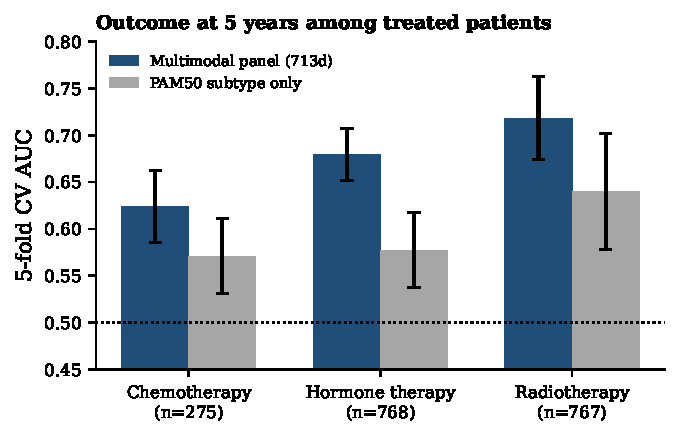
\includegraphics[width=0.7\linewidth]{figures/figF_treatment_auc.pdf}
\caption{Five-year outcome discrimination within treatment subgroups on METABRIC. The multimodal panel exceeds the PAM50 subtype-only baseline in all three cohorts, most strongly under hormone therapy.}
\label{fig:treatment}
\end{figure}

\subsection{Treatment-Response Prediction: Subtype Probabilities Track pCR, Genomic Features Add Nothing}
\label{sec:pcr}

Subtype accuracy is a surrogate endpoint. To test whether the framework carries clinical value we applied it to a genuine response endpoint: pathological complete response (pCR) after neoadjuvant chemotherapy in GSE20194 (n=278, 56 pCR / 222 residual disease, Affymetrix HG-U133A). The 412-gene panel covers 276 genes on this platform (67.0\%). We compared a clinical-only model (age, ER, PR, HER2, grade, histology) against the same model augmented with genomic features and with predicted subtype probabilities.

The genomic panel did not significantly improve on clinical features in this cohort. Clinical-only AUC was 0.791, genomic-only AUC was 0.773, and combined AUC was 0.794. The difference was \textbf{+0.0045} (95\% CI \textbf{[$-0.060$, $+0.061$]}, $P(\Delta > 0) = 0.576$). Adding predicted subtype probabilities to the clinical model gave an AUC of 0.797, a difference of $+0.0034$ (95\% CI [$-0.023$, $+0.030$]). Neither increment was distinguishable from zero. The genomic-only model had lower AUC than the clinical-only model.

What the predictions do capture is biology. Grouping patients by predicted subtype gives pCR rates that followed the observed subtype pattern: HER2-enriched 53.6\% (15/28), Basal-like 42.4\% (14/33), claudin-low 26.2\% (11/42), Luminal B 13.2\% (9/68), Luminal A 6.0\% (6/100), Normal-like 14.3\% (1/7). HER2-enriched and Basal-like had higher observed pCR rates than Luminal A. The Luminal A estimate is based on 100 patients. Predicted-subtype probabilities alone reached AUC 0.759, comparable to ER status alone (0.727).

We report this as a negative result. In this cohort, the genomic panel did not improve pCR prediction beyond routine clinical variables, including receptor status and grade. Its observed value in this study was prognostic rather than predictive. This is consistent with the related analysis in Section~\ref{sec:route_a_treatment}, where the panel out-discriminates a subtype-only baseline for \emph{outcome} within treated subgroups while METABRIC records treatment administration rather than response.

\begin{figure}[htbp]
\centering
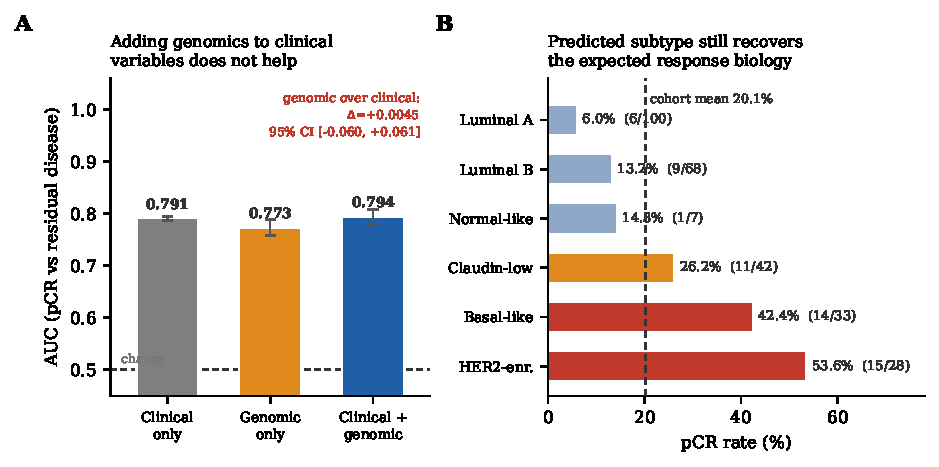
\includegraphics[width=0.85\linewidth]{figures/figI_pcr.pdf}
\caption{Treatment-response prediction in GSE20194 (n=278; 56 pCR, 222 residual disease). \textbf{(A)} Discrimination of pCR after neoadjuvant chemotherapy. The genomic panel does not improve on clinical variables: the increment is $+0.0045$ with a 95\% CI spanning zero, and the genomic-only model (0.773) is worse than clinical-only (0.791). \textbf{(B)} pCR rate by predicted subtype. Despite adding no predictive value over clinical features, the predicted subtype reproduces the observed response pattern, with pCR rates of 53.6\% for HER2-enriched and 42.4\% for basal-like compared with 6.0\% for Luminal A.}
\label{fig:pcr}
\end{figure}

\section{Methodological Investigation: A Fusion Transformer Does Not Improve PAM50 Prediction}
\label{sec:route_a}

The preceding results establish a linear reference: multinomial logistic regression over
clinical, mRNA and methylation features, reaching 75.3\% cross-validated accuracy. We
tested whether a multimodal fusion architecture could exceed it. The architecture
projects each modality into a shared space and combines them through cross-modal
attention. Capacity, regularization, pretraining, and external-validation experiments
produced a negative result. We report it here in condensed form because it is a caution
about evaluation practice rather than a competing contribution; the full results are in
Supplementary Section~S1.

\subsection{The Gap Is Bias-Limited, Not Optimization-Limited}
\label{sec:route_a_bias}

We swept model capacity across 12 configurations ($d \in \{32,64,128,256\} \times
L \in \{1,2,4\}$) under the same 5-fold protocol as the linear reference. All twelve land
between 65.5\% and 69.8\% (Supplementary Figure S1), eleven of them within a 4-point band,
with the best at $d$=128, $L$=4 -- still 5.5 points below the reference. Capacity is
therefore not the binding constraint. A learning curve on the best small configuration
(Supplementary Figure S2) rises 62.2\%, 64.7\%, 66.5\% and 68.0\% at $n$ = 240, 479, 718
and 958; fitting $\text{acc}(n) = a + b\ln n$ gives $b = 4.10$ and projects that
\textbf{5,939 samples} -- 6.2 times the present training set -- would be needed for parity.
A variance problem is fixed by more data or stronger regularization; a bias problem only by
changing the hypothesis class. The architecture's irreducible performance sits below the
linear model's, so our working conclusion is that cross-modal attention is a poorer
inductive bias than a linear combination on this problem, where 713 features describe 958
patients and the copy-number and mutation blocks carry little signal.

\subsection{Other Interventions Did Not Close the Gap}
\label{sec:route_a_reg}

Five regularization axes (modality dropout, weight decay, label smoothing, feature
dropout, reduced width with depth) were swept under the same protocol (Supplementary
Figure S3). The strongest single axis, modality dropout at 0.2, moves the baseline from
67.7\% to 68.6\%, a gain of 0.84 points; the best two-axis combination reaches 68.1\%, no
better than the best single axis. Every configuration remains roughly 7 points below the
reference, corroborating the bias reading: the deficit is not recoverable by constraining
the optimizer's search.

The one intervention that produced a real internal gain was self-supervised pretraining,
where the modality encoders reconstruct a randomly masked 30\% of their own features. To
keep the estimate honest the encoder is pretrained \emph{separately within each
cross-validation fold}, on that fold's training portion only. This raised cross-validated
accuracy from 67.3\% to 70.0\% (Supplementary Figure S4), the best result any Transformer
variant achieved in the study. It did not survive external validation.

\subsection{External Validation Reverses the Ranking}
\label{sec:route_a_tcga}

All three models were evaluated on TCGA-BRCA (n=987) with within-platform rank
normalization, and each carried through to a survival C-index (Cox model fitted on
METABRIC, applied unchanged to TCGA).

\begin{table}[htbp]
\centering
\caption{Internal versus external performance for the mRNA-only reference and two
Transformer variants, all on the 412-gene panel under the same normalization protocol.}
\label{tab:route_a}
\fitcol{%
\begin{tabular}{lccc}
\toprule
\textbf{Model} & \textbf{METABRIC CV} & \textbf{TCGA acc.} & \textbf{TCGA C-idx} \\
\midrule
Logistic regression (ref.) & 75.3\% & 73.8\% & 0.577 \\
Fusion Transformer & 67.3\% & 66.1\% & 0.551 \\
\quad + pretraining & \textbf{70.0\%} & 62.7\% & 0.530 \\
\bottomrule
\end{tabular}}
\end{table}

The ranking reverses. The pretrained Transformer, which had the best internal score, falls
to 62.7\% -- \emph{worse} than the unguided model -- an internal-to-external drop of 7.3
points against 1.2 points for the unguided Transformer and 1.5 for the reference, with the
same ordering in survival C-index. Pretraining on METABRIC's masked-feature distribution
teaches the encoder to exploit covariance structure specific to that cohort: it becomes a
better METABRIC model, not a better model of breast cancer. Under cross-validation the
effect looks like genuine improvement because the held-out fold is drawn from the same
distribution, and only external validation separates the two interpretations. This is the
reason we report the Transformer as a negative result, and why we do not adopt it as the
paper's method.

Two additional results, given in full in Supplementary Section~S1, are consistent. On a
second external cohort (GSE21653, n=266) the reference reaches 63.2\% and the external
survival C-index is 0.584, close to TCGA's 0.577, so the \emph{discrimination} transfers
even though absolute accuracy does not; the accuracy loss is concentrated in the
basal-like class, which is 28\% of that cohort against 10\% of the training set. Pooling
GSE21653 into training (1,224 samples) raises the unguided Transformer by 1.11 points
against a learning-curve prediction of 1.00 point, while the reference and the pretrained
model both lose about 1 point: the same bias--variance account from the opposite
direction.

\section{Discussion}

Our primary contribution is an empirical analysis of how annotation-space differences affect cross-cohort evaluation of breast cancer molecular-subtype classifiers. We do not propose a new label-shift estimator. Instead, we show that applying an externally specified PAM50 label space changes reported scores for two cohorts, and that this operation must be distinguished from improving the classifier itself.

\textbf{The effect depends on the metric and cohort.} TCGA-BRCA accuracy (73.76\%) was nearly identical to METABRIC test accuracy (73.8\%), so these data do not show an accuracy transfer gap for TCGA before reconciliation. However, six-class macro F1 on TCGA was 0.585, compared with 0.702 when averaged over its five annotated classes. On GSE21653, baseline accuracy was 63.16\%, and the combined PAM50 restriction plus EM correction yielded 74.06\%. These observations support a narrower conclusion: cross-cohort metrics can change when the evaluation label space is reconciled, while residual differences may also reflect platform, prevalence, sample composition, or other cohort effects. The patterns observed here are specific to the studied cohorts and label spaces and should not be generalized without further validation.

\textbf{The tested procedures did not recover the label space from unlabeled predictions.} Unconstrained EM retained an estimated prior of 0.0751 for claudin-low on TCGA-BRCA, although that class is absent under PAM50 annotation. The geometric detector had low simulated detection F1 under both scorings ($0.047$ originally, $0.232$ under the standard empty-set convention), and the BIC procedure selected a non-empty absent set in 90\% of clean null runs; the uncalibrated EM rule that ranked best of the six after re-scoring still flags clean cohorts once prior shift is present. These results show that the tested procedures did not reliably identify the annotation space at these sample sizes. They do not establish a general impossibility theorem for every classifier or detector. In practice, the allowed target labels should be specified from cohort documentation, rather than inferred from these predictions alone.

\textbf{Separating label-space and prior changes matters.} In the controlled simulation, the correction changed accuracy by $-0.4$ to $+3.2$ points without prior shift and by $+5.9$ to $+7.9$ points when prior shift was also present. These results indicate that the effects can interact under the tested settings. They should not be read as calibrated estimates for an unobserved clinical cohort.

\textbf{Modality selection is internal, and the multimodal advantage does not transfer.} The three-modality model (clinical, mRNA, and methylation) outperformed the five-modality model in the reported METABRIC split and cross-validation, but this comparison is internal to METABRIC. When we rebuilt a reduced three-layer space that both cohorts carry and repeated the ablation there (Section~\ref{sec:external_multimodal}), methylation produced no cross-validated gain and lowered external accuracy by 1.9 points, while the harmonized clinical block gained 2.4 points on the METABRIC test set and moved external accuracy by at most 0.3 points; no configuration differed significantly from mRNA alone. The internal advantage of the original 713-dimension model rests on 59 METABRIC-specific clinical dimensions with no external counterpart, so the best internal model is the one that cannot be transported. Low SHAP attribution for copy-number and mutation features is consistent with limited contribution in this fitted model, but does not establish that these modalities are uninformative elsewhere. The practical implication is that modality selection should be decided on a cohort that shares the target's schema, or reported explicitly as an internal result.

\textbf{Rank normalization handles the feature side; it does not handle the label side.} The within-platform rank normalization strategy transfers the feature distribution across platforms without retraining: with it, TCGA-BRCA holds its METABRIC accuracy despite the shift from microarray to RNA-seq, whereas METABRIC-statistic standardization collapses it to 20.7\%. That result is real but partial, and our analysis shows why. Normalization operates on features and is therefore blind to a mismatched label space; the two failures are orthogonal and require different remedies. What transfers most cleanly across all three cohorts is the survival risk signal (C-index 0.577 and 0.584 on the external cohorts, against 0.598 internally), because discrimination of risk does not depend on the class label being well-calibrated to a local annotation standard. Practically, we would deploy the rank-normalized model with an explicit per-cohort label-space declaration, and treat survival discrimination rather than subtype accuracy as the more portable endpoint.

\textbf{Relationship to established PAM50 assays.} We do not claim a head-to-head comparison against Prosigna, and one is not possible: Prosigna is a locked RT-qPCR assay whose classifier, normalisation and decision thresholds are not public, so it cannot be executed on the expression matrices used here. What the external cohorts supply is the PAM50 call itself, assigned by the originating studies, and that call is the target our model is scored against -- the 73.8\% on TCGA and 63.2\% on GSE21653 therefore measure agreement with the reference standard, not superiority over it. The relevant published benchmark is the inter-platform concordance of PAM50 calls, which is itself imperfect \cite{bastien2012pam50}, and part of the gap we report is plausibly attributable to that, particularly at the Luminal A/B boundary.

\textbf{Luminal A/B confusion.} Confusion between Luminal A and Luminal B subtypes is a known challenge \cite{bastien2012pam50}. These subtypes share ER-positive status and differ primarily in proliferation-related gene expression. The 24\% Luminal B-to-Luminal A misclassification rate suggests that proliferation-specific markers such as Ki-67 could improve discrimination.

\textbf{Clinical implications.} The predicted subtypes show statistically significant but modest prognostic stratification (C-Index 0.598, $p = 0.0008$ in METABRIC; 0.577 and 0.584 in external cohorts). While these discrimination levels are below those of established clinical tools such as Oncotype DX (typically C-index 0.65--0.75), the hazard ratios align with established prognostic rankings: Luminal B, HER2-enriched, and Basal-like subtypes show elevated mortality risk relative to Luminal A \cite{prat2014research}. The value of this model lies not in replacing existing prognostic tools but in providing a methodological framework for evaluating how annotation standards affect cross-cohort comparability.

\textbf{Attention-based fusion did not improve the tested models.} We tested the obvious objection to a linear model -- that it cannot capture interactions between modalities -- by building a cross-modal attention architecture and giving it every reasonable opportunity to succeed. It did not: capacity sweeps, learning curves, five regularization axes and self-supervised pretraining all failed to bring it to parity, and the diagnosis is specific. The deficit is a bias limitation, not a variance limitation, so with 713 features and 958 training patients a linear combination is the better-matched hypothesis class in these experiments. The most instructive outcome is the reversal under external validation: pretraining produced the largest internal gain of any intervention (+2.7 points) and the largest external loss ($-$3.4 points relative to the unguided model), because a cross-validated improvement is not evidence of a better model of biology when the held-out data come from the same cohort. The same reasoning weakens any internal-only claim for deep fusion models in this domain, where cohorts in the low thousands of samples are the norm. Details are in Section~\ref{sec:route_a}.

\textbf{Panel value beyond the subtype call.} Among treated patients, the 713-dimension panel out-discriminated a PAM50-subtype-only baseline in all three treatment cohorts, most strongly for hormone therapy ($+0.102$ AUC). Since the subtype call already encodes the dominant prognostic axis, this increment indicates that within-subtype molecular variation carries prognostic information the label discards -- a clinically motivated use of the panel that does not depend on the Transformer. The finding is bounded by an important caveat: METABRIC records treatment administration rather than response, so these are prognosis estimates within treated subgroups, not predictions of therapeutic response.

\textbf{A five-class model is an equally valid design.} Because the label-space mismatch is created by training on six classes and evaluating against five, one may ask why we did not simply train on five. We tested this (Section~\ref{sec:fiveclass}): on TCGA-BRCA the five-class model matches the six-class estimator with correction ($p = 0.50$), while on GSE21653 the corrected six-class estimator is significantly better because EM additionally re-estimates a target prior that departs substantially from the source. The methodological point survives either way -- a six-class score reported against a five-class standard understates performance -- but the practical recommendation is narrower than it first appears: when the target label space is known, either design is defensible, and the choice should be made explicitly rather than by default.

\textbf{Limitations.} First, the model was developed on METABRIC and ancestry-specific performance was not assessed. Second, the real-cohort analysis covers one absent class, claudin-low, in two PAM50-annotated cohorts; the simulation extends this to every class and class pair under three absence modes (Supplementary Section~S5), but those are synthetic targets and the magnitudes there are not forecasts for a named cohort. Third, detector results apply to the tested methods and sample sizes; the controlled simulation uses Gaussian-mixture surrogates rather than expression data and is not a forecast for a new cohort. Fourth, the multimodal model was evaluated externally only in a reduced shared space. Of the 69 METABRIC clinical dimensions, 59 have no counterpart in the TCGA schema, so Section~\ref{sec:external_multimodal} substitutes a 10-field clinical block and accepts a 2.75-point internal penalty relative to the original model in order to obtain a transportable comparison; the resulting negative result concerns that reduced configuration plus the mRNA and methylation blocks, not every possible multimodal design. Finally, the training sample size may constrain nonlinear models. The SHAP analysis itself is not a limitation in this respect: the explainer is exact for the fitted linear model, so the attributions faithfully describe it. What the attributions do not support is any claim about the modalities' biological value -- a low attribution for copy-number and mutation features records their limited contribution \emph{within this fitted model and feature encoding}, not that those blocks are uninformative in general.

\section{Conclusion}

Our findings show that, in the studied cohorts, cross-cohort subtype metrics can depend on whether the evaluation label space matches the target cohort's annotation standard. Accuracy on TCGA-BRCA was similar to the METABRIC test accuracy, but the six-class macro F1 included a zero score for the absent claudin-low class. On GSE21653, restricting predictions to PAM50 classes and applying EM prior correction increased accuracy from 63.16\% to 74.06\%. These operations change how predictions are evaluated; they do not improve the classifier's learned representation. The tested unconstrained EM and absent-class detectors did not reliably recover the target label space from unlabeled predictions. Cohort comparisons should therefore report the annotation-defined label space and the metric's class set explicitly.

The multimodal METABRIC model achieved 75.3\% $\pm$ 2.6\% cross-validated accuracy and 73.8\% test accuracy. Survival discrimination was similar across the two external cohorts (C-index 0.577 and 0.584), and in a reduced three-layer space shared with TCGA-BRCA the internal multimodal advantage did not transfer: no configuration beat mRNA alone significantly, and the best internal model depended on 59 METABRIC-specific clinical dimensions. Cross-modal attention fusion did not outperform the linear reference in the tested experiments, and the internal gain from pretraining did not transfer to TCGA. These findings are limited to the studied cohorts, label spaces, and model configurations, and should not be generalized without further validation.

\section*{Declarations}
\textbf{Data availability:} METABRIC and TCGA-BRCA are available through cBioPortal (\url{https://www.cbioportal.org/}). GEO accession records are available for GSE21653 and GSE20194. Redistribution of processed data should follow the terms of the source repositories.

\textbf{Code availability:} The code and preprocessed data used for the analyses in this manuscript are available at \href{https://github.com/HAHA12345677888/pam50-label-space}{GitHub}. A versioned snapshot will be archived at \href{https://zenodo.org}{Zenodo} with a DOI prior to submission; that archive will pin the exact revision used for the reported results.

\textbf{Author contributions:} Suxing Liu contributed to the study conception, data analysis, and manuscript preparation. Zhijian Zheng and Jiahao Wang contributed to the analysis and to critical revision of the manuscript. All authors read and approved the final manuscript.

\textbf{Funding:} Funding information has not been provided.

\textbf{Competing interests:} The authors declare no competing interests.

\textbf{Ethics approval and consent to participate:} The analyses use public cohort resources. The analyses were conducted in compliance with institutional review requirements for publicly available datasets.

\textbf{Correspondence:} Correspondence and requests for materials should be addressed to Suxing Liu (email: liushuxing8888@student.usm.my).

\bibliographystyle{IEEEtran}
\bibliography{references}

\end{document}
